\documentclass[a4paper,12pt,onecolumn]{article}

\usepackage[T1]{fontenc}
\usepackage[utf8]{inputenc}
\usepackage[english]{babel}
\usepackage{amssymb,amsmath,amsthm,array,epsfig,lmodern,gensymb,pstricks,subfig,
hyperref,verbatim,booktabs,textcomp}
\usepackage[notref,notcite]{showkeys}

\newcommand{\R}{\mathbb R}
\newcommand{\D}{\mathcal D}
\newcommand{\W}{\vec{\mathcal W}}
\newcommand{\vol}{\mathcal{L}^d}
\newcommand{\surfvol}{\mathcal{H}^{d-1}}
\newcommand{\dH}[1]{\;{\rm d}{\cal H}^{#1}} % Hausdorff measure
\newcommand{\dL}[1]{\;{\rm d}{\cal L}^{#1}} % Lebesgue measure
\newcommand{\bigchi}{\ensuremath{\mathrm{\mathcal{X}}}}
\newcommand{\charfcn}[1]{\bigchi_{#1}} % characteristic function
\newcommand{\Vh}{\underline{V}(\Gamma^m)}
\newcommand{\Wh}{W(\Gamma^m)}
\newcommand{\Vht}{\underline{V}(\Gamma^h(t))}
\newcommand{\Wht}{W(\Gamma^h(t))}
\newcommand{\uspacesimple}{\mathbb{U}}
\newcommand{\uspace}[1]{\mathbb{U}(\vec{#1})}
\newcommand{\uspacedisc}[2]{\mathbb{U}^{#2}(\vec{#1})}
\newcommand{\pspace}{\mathbb{P}}
\newcommand{\pnormspace}{\widetilde\pspace} % normalized pressure space
\newcommand{\uspacesimpleref}{\mathcal{U}} % ale reference space
\newcommand{\uspaceref}[1]{\mathcal{U}(\vec{#1})} % ale reference space
\newcommand{\uspacesemidiscref}[2]{\mathcal{U}^{#2}(\vec{#1})}
% ale reference space
\newcommand{\pspaceref}{\mathcal{P}} % ale reference space
\newcommand{\pnormspaceref}{\widetilde\pspaceref}% ale reference space
\newcommand{\uspacesimpleale}{\mathfrak{U}} % ale space
\newcommand{\uspaceale}[1]{\mathfrak{U}(\vec{#1})} % ale space
\newcommand{\uspacesemidiscale}[3]{\mathfrak{U}^{#2}(\vec{#1},#3)} % ale space
\newcommand{\uspacediscale}[2]{\mathfrak{U}^{#2}(\vec{#1})} % ale space
\newcommand{\pspaceale}{\mathfrak{P}} % ale space
\newcommand{\pnormspaceale}{\widetilde\pspaceale}% ale normalized space
\newcommand{\kspace}{\mathbb{K}}
\newcommand{\xspace}{\mathbb{X}}
\newcommand{\sigmaO}{o}
\newcommand{\nabs}{\nabla_{\!s}}
\newcommand{\id}{\rm id}
\newcommand{\ddt}{\frac{\rm d}{{\rm d}t}}
\newcommand{\NbulkT}{\vec{N}_{\Gamma,\Omega}^T}
\newcommand{\Nbulk}{\vec{N}_{\Gamma,\Omega}}
\newcommand{\errorXx}{\|\Gamma^h - \Gamma\|_{L^\infty}}
\newcommand{\LerrorUu}[1]{\|\vec U - I^h_{#1}\,\vec u\|_{L^2}}
\newcommand{\HerrorUu}[1]{\|\vec U - I^h_{#1}\,\vec u\|_{L^2(H^1)}}
\newcommand{\LerrorPp}{\|P - p\|_{L^2}}
\newcommand{\unitn}{\vec{\rm n}}
\newcommand{\unitt}{\vec{\rm t}}
\newcommand{\mat}[1]{\underline{\underline{#1}}\rule{0pt}{0pt}}
\newcommand{\Rey}{\mbox{\textit{Re}}} % Reynolds number
\newcommand{\V}{\vec{\mathcal{V}}} % surface velocity
\newcommand{\pdg}{${\rm P1}^{{\rm dg}_\Gamma}$} % P1 DG across interface
\newcommand{\strikes}{\mbox{$s\!\!\!\!\:/$}}
\newcommand{\myurl}[1]{\hfil\penalty 100 \hfilneg \hbox{\url{#1}}} % force
% newline before long url

\newcommand{\schemeAex}{{\mathcal{A}^h_{\rm ex}}}
\newcommand{\schemeAim}{{\mathcal{A}^h_{\rm im}}}
\newcommand{\schemeB}{{\mathcal{B}^h}}
\newcommand{\schemeALE}{{\mathcal{C}^h_{\rm ALE}}}

\newtheorem{thm}{Theorem}
\newtheorem{lem}[thm]{Lemma}
\newtheorem{rem}[thm]{Remark}

\newenvironment{keywords}{{\upshape\bfseries Key words. }\ignorespaces}{}

\renewcommand{\theequation}{\arabic{section}.\arabic{equation}}

%\textwidth 425pt
\textwidth 455pt \oddsidemargin 0pt \evensidemargin 0pt \headsep
0pt \headheight 0pt \textheight 655pt \parskip 10pt

\title{Fitted front tracking methods for two-phase incompressible 
Navier--Stokes flow: \\
Eulerian and ALE finite element discretizations
}
\author{Marco Agnese and Robert N\"urnberg%
\thanks{email: \texttt{\{m.agnese13,robert.nurnberg\}@imperial.ac.uk}}\\
\small
Department of Mathematics, Imperial College, London, SW7 2AZ, U.K.}
\date{}

\begin{document}

\captionsetup[subfigure]{labelformat=empty} % remove label subplot

\maketitle

\begin{abstract}
We investigate novel fitted finite element approximations for two-phase
Navier--Stokes flow. In particular, we consider both Eulerian and
Arbitrary Lagrangian--Eulerian (ALE) finite element formulations.
The moving interface is approximated with the help of piecewise linear
finite element functions. The bulk mesh is fitted to the interface
approximation, so that standard bulk finite element spaces can be used
throughout.
The meshes describing the discrete interface in
general do not deteriorate in time, which means that in numerical simulations a
smoothing or a remeshing of the interface mesh is not necessary.
We present several numerical experiments for the various numerical methods,
which demonstrate the accuracy and robustness of the proposed algorithms.
We also compare the accuracy and efficiency of the Eulerian and ALE
formulations.
\end{abstract}

\begin{keywords}
incompressible two-phase flow, Navier--Stokes equations, ALE method,
free boundary problem, surface tension, finite elements, front tracking
\end{keywords}

\section{Introduction}\label{sec:introdution}
Fluid flow problems with a moving interface are encountered in many
applications in physics, engineering and biophysics. Typical applications 
include drops and bubbles, die swell, dam break, liquid storage tanks, 
ink-jet printing and fuel injection. For this reason, developing robust and
efficient numerical methods for these flows is an important problem and
has attracted tremendous interest over the last few decades.

A crucial aspect of these types of fluid flow problems is that apart from 
the solution of the flow in the bulk domain, the position of the interface
separating the two bulk phases also needs to be determined. 
At the interface certain boundary conditions need to be fulfilled, which
specify the motion of the phase boundary. 
These conditions relate the variables of the bulk flow, velocity and pressure, 
across the two phase, taking into account external influences, such as for 
example surface tension. Numerically, in order
to be able to compute the flow solution as well as the interface
geometry, a measure to track the interface starting from an initial position
needs to be incorporated.
There are several strategies to deal with this problem, which can be divided 
into two categories depending on the viewpoint: interface capturing and 
interface tracking.

Interface capturing methods use an Eulerian description of the interface, which
is defined implicitly. A characteristic scalar field,
that is advected by the flow, is used to identify
the two phases as well as the interface along the boundaries of the individual
fluid domains. Depending on the method, this scalar field may be, for example,
a discontinuous Heaviside function or a signed-distance function. The most
important methods, which belong to this category, are the particle method,
the volume-of-fluid method, the level-set method and the phase-field method.
The particle method utilizes mass-less particles distributed in an Eulerian
mesh to capture the fluid flow and in particular the interface position, see
e.g \cite{Girault1976}. In the volume-of-fluid method, the characteristic
function of one of the phases is approximated numerically, see e.g.
\cite{HirtN81,RenardyR02,Popinet09}. In the level-set method, the interface is
given as the level set of a function, which has to be determined, see e.g.
\cite{SussmanSO94,Sethian99,OsherF03,GrossR07,GrossR11,Svacek17}. Instead, the
phase-field method works with diffuse interfaces, and therefore the transition
layer between the phases has a finite size. There is no tracking mechanism for
the interface, but the phase state is included implicitly in the governing
equations. The interface is associated with a smooth, but highly localized
variation of the so-called phase-field variable. We refer to
\cite{HohenbergH77,AndersonMW98,LowengrubT98,Feng06,KaySW08,AbelsGG12,GrunK14}
for details. 
The appeal of interface capturing approaches is the fact that they are usually
easy to implement, and that they offer an automated way to deal with
topological changes.
%In general, the great advantage of the interface capturing
%approaches is that they are inherently able to deal with topological changes of
%the interface. This allows a much more flexible interface description than in
%interface tracking approaches. On the other hand, it is challenging to treat
%accurately discontinuous quantities across the interface, to have mass
%conservation within each phase and to apply boundary conditions along the
%interface.

Interface tracking approaches, instead, use a Lagrangian description of the
interface which is described explicitly. Here the interface is represented
by a collection of particles or points, and this representation is
transported by the bulk flow velocity. 
The great
advantage of interface tracking approaches is that they offer an accurate and
computationally efficient approximation of the evolving interface. 
Challenges are the mesh quality both of the interface representation and of the
bulk triangulations, as well as the need to heuristically deal with topological
changes.
We refer e.g.\ to
\cite{UnverdiT92,Bansch01,Tryggvason_etal01,GanesanT08,spurious,
fluidfbp} for further details, and to \cite{LevequeL97,Peskin02} for the
related immersed boundary method, which is used to simulate fluid-structure
interactions using Eulerian coordinates for the fluid and Lagrangian
coordinates for the structure.

In this paper we use a direct description of the interface using a
parameterization of the unknown interface, similarly to the previous work
\cite{fluidfbp}. In particular, our numerical method will be based
on a piecewise linear parametric finite elements, and the description of the
interface will be advected in normal direction
with the normal part of the fluid velocity. The tangential degrees
of freedom of the interface velocity are implicitly used to ensure a 
good mesh quality, and this is a main feature of our proposed methods. 
But in contrast to \cite{fluidfbp}, where an unfitted bulk finite element 
approximation was used, we will adopt a fitted mesh approach, which means 
that the discrete interface is composed of faces of elements from the bulk 
triangulation. A fitted method has the advantage that discontinuity jumps 
at the interface are captured naturally, but it has the disadvantage that in
a standard Eulerian method the velocity needs to be interpolated from
an old mesh to a new mesh, unless the interface is stationary. Hence so-called
Arbitrary Lagrangian Eulerian (ALE) methods are often proposed. Here
the equations are posed in a moving domain framework,
and an arbitrary Lagrangian velocity may be chosen to improve the quality of
the bulk mesh. The original idea for ALE methods goes back to 
the papers \cite{Donea83,Hughes81}, and we refer to
\cite{Nobile99,NobilePhd,Formaggia04,Ganesan06,GanesanT08} for applications 
to two-phase Navier--Stokes flow.

In this paper we will proposed both standard Eulerian and
ALE finite element approximations for two-phase incompressible Navier--Stokes
flow. One aim of our paper is to investigate numerically, if there is a clear
advantage of ALE type methods over standard Eulerian methods.
We note that in the case of viscous incompressible two-phase Stokes flow, 
there is no need for the numerical method to interpolate the velocity from the
old to the new mesh. Hence there is no need to employ an ALE method. In fact,
in the case of two-phase Stokes flow, our proposed numerical methods collapse
the the approximation considered by the authors in 
\cite{stokesfitted}.



The remainder of the paper is organized as follows.
\footnote{TODO}

\section{Mathematical model and weak formulations}\label{sec:ns_model}
Let $\Omega\subset\R^d$, for $d=2$ or $d=3$ be a given domain that contains two
different immiscible, incompressible fluids (liquid-liquid or liquid-gas) which
for all $t\in[0,T]$ occupy time dependent regions $\Omega_+(t)$ and
$\Omega_-(t):=\Omega\setminus\overline{\Omega}_+(t)$ and which are separated by
an interface $(\Gamma(t))_{t\in[0,T]}$, $\Gamma(t)\subset\Omega$. We limit
ourselves to interfaces formed by closed hypersurfaces, see
Figure~\ref{fig:two_phase_sketch} for a pictorial representation in the case
$d=2$.
\begin{figure}
\begin{center}
\unitlength15mm
\psset{unit=\unitlength,linewidth=1pt}
\begin{picture}(4,4)(0,0)
\psline(0,0)(4,0)(4,4)(0,4)(0,0)
\psellipse(2,2)(1,1)
\psline{->}(3,2)(3.5,2)
\put(3.25,1.75){$\vec\nu$}
\put(1.75,0.75){{$\Gamma(t)$}}
\put(1.75,2){{$\Omega_-(t)$}}
\put(0.5,3.25){{$\Omega_+(t)$}}
\end{picture}
\end{center}
\caption{The domain $\Omega$.}
\label{fig:two_phase_sketch}
\end{figure}
For later use, we assume that $(\Gamma(t))_{t\in [0,T]}$ is a sufficiently
smooth evolving hypersurface without boundary that is parameterized by
$\vec x(\cdot,t):\Upsilon\to\R^d$, where $\Upsilon\subset \R^d$ is a given
reference manifold such that $\Gamma(t) = \vec x(\Upsilon,t)$. Then
\begin{equation} \label{eq:V}
\V(\vec z, t) := \vec x_t(\vec q, t) \quad
\forall\ \vec z = \vec x(\vec q,t) \in \Gamma(t)\,,
\end{equation}
defines the velocity of $\Gamma(t)$, and $\V \,.\,\vec \nu$ is
the normal velocity of the evolving hypersurface $\Gamma(t)$,
where $\vec\nu(t)$ is the unit normal on $\Gamma(t)$ pointing into
$\Omega_+(t)$.

Denoting the velocity and pressure by $\vec u$ and $p$, respectively, we
introduce the stress tensor
\begin{equation} \label{eq:stress_tensor}
\mat\sigma = \mu \,(\nabla\,\vec u + (\nabla\,\vec u)^T) - p\,\mat\id
= 2\,\mu\, \mat D(\vec u)-p\,\mat\id\,,
\end{equation}
where $\mu(t) = \mu_+\,\charfcn{\Omega_+(t)} + \mu_-\,\charfcn{\Omega_-(t)}$,
with $\mu_\pm \in \R_{>0}$, denotes the dynamic viscosities in the two phases,
$\mat\id \in \R^{d \times d}$ is the identity matrix and
$\mat D(\vec u):=\frac12\, (\nabla\vec u+(\nabla\vec u)^T)$
is the rate-of-deformation tensor. Here and throughout, $\charfcn{\D}$ denotes
the characteristic function for a set $\D$.

The fluid dynamics in the bulk domain $\Omega$ is governed by the two-phase
Navier--Stokes model
\begin{subequations}
\begin{alignat}{2}
\rho\,(\vec u_t +(\vec u \,.\, \nabla)\vec u) -2 \mu\,\nabla\,.\,\mat D(\vec u)+
\nabla\,p & = \vec f \quad &&\mbox{in } \Omega_\pm(t)\,,
\label{eq:ns_momentum_bis} \\
\nabla\,.\,\vec u & = 0 \quad &&\mbox{in } \Omega_\pm(t)\,,
\label{eq:ns_mass_bis}
\end{alignat}
\end{subequations}
where $\rho(t) = \rho_+\,\charfcn{\Omega_+(t)}+\rho_-\,\charfcn{\Omega_-(t)}$,
with $\rho_\pm \in \R_{>0}$, denotes the fluid density in the two phases, and 
where $\vec f:=\rho\,\vec f_1+\vec f_2$ is a possible forcing term.
The velocity and stress tensor need to be coupled across the free surface
$\Gamma(t)$. Viscosity of the fluids leads to the continuity condition
\begin{equation}\label{eq:interface_jump_velocity}
[\vec u]_-^+ = \vec 0 \quad \mbox{on } \Gamma(t)\,,
\end{equation}
where $[\vec u]_-^+ := \vec u_+ - \vec u_-$ denote the jump in velocity across
the interface $\Gamma(t)$. Here and throughout, we employ the shorthand notation
$\vec h_\pm := \vec h\!\mid_{\Omega_\pm(t)}$ for a function
$\vec h : \Omega \times [0,T] \to \R^d$; and similarly for scalar and
matrix-valued functions. The assumption that there is no change of phase leads
to the dynamic interface condition
\begin{equation}\label{eq:interface_velocity}
\V\,.\,\vec\nu = \vec u\,.\,\vec \nu \quad \mbox{on }
\Gamma(t)\,,
\end{equation}
which means that the normal velocity of the interface needs to match the flow
normal velocity across the interface $\Gamma(t)$. Moreover, the momentum
conservation in a small material volume that intersects the interface leads to
the stress balance condition
\begin{equation}\label{eq:interface_jump_stress_div}
[\mat\sigma\,\vec \nu]_-^+ = -\nabs\,.\mat\sigma_{\Gamma} \quad \mbox{on }
\Gamma(t)\,,
\end{equation}
where $\mat\sigma_{\Gamma}$ is the interface stress tensor and $\nabs\,.$ is
the surface divergence on $\Gamma(t)$. The operator $\nabs$ is the surface
gradient on $\Gamma(t)$ and it is the orthogonal projection of the usual
gradient operator $\nabla$ on the tangent space of the surface $\Gamma(t)$.
Therefore, given a smooth function $h$ defined on a neighbourhood of
$\Gamma(t)$, it is defined as
\begin{equation}\label{eq:surface_gradient}
\nabs\,h(\vec z)=\mat P(\vec z)\,\nabla\,h(\vec z)=\nabla\,h(\vec z)\,-
\,\nabla\,h(\vec z)\,.\,\vec\nu(\vec z)\,\vec\nu(\vec z)\,,\quad \vec z
\in\Gamma(t)\,,
\end{equation}
with the usual projection operator $\mat P$ defined as
\begin{equation}\label{eq:surface_projection}
\mat P=\mat\id\,-\,\vec\nu\,\vec\nu\,^T\quad \mbox{on } \Gamma(t)\,.
\end{equation}
It can be shown that the definition of $\nabs\,h$ does not depend on the chosen
extension of $h$, but only on the value of $h$ on $\Gamma(t)$. See e.g.\
\cite[\S2.1]{DeckelnickDE05} for details.
For later use, we also define the surface
Laplacian, also known as Laplace--Beltrami operator, $\Delta_s$ on $\Gamma(t)$
as
\begin{equation}\label{eq:surface_laplacian}
\Delta_s = \nabs\,.\,\nabs\,.
\end{equation}
We restrict ourselves to the case that the only force acting on the interface
is the surface tension contact force. Therefore the interface stress tensor
$\mat\sigma_\Gamma$ has the following constitutive equation
\begin{equation}\label{eq:interface_stress_tensor}
\mat\sigma_{\Gamma}=\gamma\,\mat P\,,
\end{equation}
where $\gamma$ is the surface tension coefficient. Substituting
(\ref{eq:interface_stress_tensor}) in (\ref{eq:interface_jump_stress_div}) we
obtain, assuming $\gamma$ is constant, the so called clean interface model for
the interfacial forces
\begin{equation}
[\mat\sigma\,\vec \nu]_-^+ = -\gamma\,\varkappa\,\vec\nu \quad \mbox{on }
\Gamma(t)\,,
\end{equation}
which, in the case of Newtonian stress tensor (\ref{eq:stress_tensor}), assumes
the form
\begin{equation}\label{eq:interface_jump_stress}
[2\mu \,\mat D(\vec u)\,.\,\vec\nu - p\,\vec \nu]_-^+
= -\gamma\,\varkappa\,\vec\nu \quad \mbox{on } \Gamma(t)\,.
\end{equation}
Here $\varkappa$ denotes the mean curvature of $\Gamma(t)$, i.e.\ the sum of
the principal curvatures of $\Gamma(t)$, where we have adopted the sign
convention that $\varkappa$ is negative where $\Omega_-(t)$ is locally convex.
In particular, see e.g.\ \cite{DeckelnickDE05}, it holds that
\begin{equation} \label{eq:LBop}
\Delta_s\, \vec \id = \varkappa\, \vec\nu \qquad \mbox{on $\Gamma(t)$}\,.
\end{equation}

In order to close the system, we prescribe the
initial data $\Gamma(0) = \Gamma_0$ and the initial velocity
$\vec u(0) = \vec u_0$. Finally, we impose the Dirichlet condition $\vec u =
\vec g$ on $\partial_1 \Omega$ and the free-slip condition $\vec u \,.\,\unitn =
0$ and $\mat\sigma\,\unitn\,.\,\unitt = 0$, $\forall \unitt \in
\{\unitn\}^\perp$, on $\partial_2 \Omega$, with $\unitn$ denoting the outer
unit normal of $\partial \Omega$ and $\{\unitn\}^\perp := \{ \unitt \in \R^d :
\unitt \,.\,\unitn = 0\}$. As usual, it holds that
$\partial\Omega =\partial_1\Omega \cup \partial_2\Omega$ and $\partial_1\Omega
\cap \partial_2\Omega = \emptyset$. Therefore the total system of equations
can be rewritten as follows:
\footnote{Marco: Are these the right boundary conditions? What about free-slip?}
\begin{subequations}
\begin{alignat}{2}
\rho\,(\vec u_t +(\vec u \,.\, \nabla)\vec u) -2 \mu\,\nabla\,.\,\mat D(\vec u)+
\nabla\,p & = \vec f
\quad &&\mbox{in } \Omega_\pm(t)\,, \label{eq:ns_full_momentum} \\
\nabla\,.\,\vec u & = 0 \quad &&\mbox{in } \Omega_\pm(t)\,,
\label{eq:ns_full_mass} \\
\vec u & = \vec g \quad &&\mbox{on } \partial_1\Omega\,,
\label{eq:ns_full_dirichlet} \\
\vec u \,.\,\unitn = 0 \,,\quad \mat\sigma\,\unitn\,.\,\unitt & = 0
\quad\forall \unitt \in \{\unitn\}^\perp \quad && \mbox{on } \partial_2\Omega\,,
\label{eq:ns_full_freeslip}\\
[\vec u]_-^+ & = \vec 0 \quad &&\mbox{on } \Gamma(t)\,,
\label{eq:ns_full_jump_velocity} \\
[2\mu \,\mat D(\vec u)\,.\,\vec\nu - p\,\vec \nu]_-^+
& = -\gamma\,\varkappa\,\vec\nu
\quad &&\mbox{on } \Gamma(t)\,, \label{eq:ns_full_jump_stress} \\
(\V-\vec u)\,.\,\vec \nu & = 0
\quad &&\mbox{on } \Gamma(t)\,,\label{eq:ns_full_velocity}  \\
\Gamma(0) & = \Gamma_0 \,,\label{eq:ns_full_initial_interface} \\
\vec u(0) & = \vec u_0 \,.\label{eq:ns_full_initial_velocity}
\end{alignat}
\end{subequations}
In what follows we introduce different weak formulations for
(\ref{eq:ns_full_momentum}--i), on which our finite element approximations will
be based.

\subsection{Eulerian weak formulations}\label{sec:ns_weak}
In order to obtain a weak formulation for (\ref{eq:ns_full_momentum}--i), 
we define the function spaces, for a given $\vec b \in [H^1(\Omega)]^d$,
\begin{align*}
\uspace b &:= \{\vec \phi\in[H^1(\Omega)]^d:
\vec \phi =\vec b\quad \mbox{on }\partial_1\Omega\,,
\quad \vec \phi\,.\,\unitn=0 \quad \mbox{on }\partial_2\Omega\}\,,\\
\pspace &:= L^2(\Omega)\,,\qquad
\pnormspace := \{\eta\in\pspace : \int_\Omega\eta\dL{d}=0 \}\,,
\end{align*}
and let, as usual, $(\cdot,\cdot)$ and $\langle \cdot, \cdot
\rangle_{\Gamma(t)}$ denote the $L^2$--inner products on $\Omega$ and
$\Gamma(t)$, respectively. In addition, we let $\vol$ and $\surfvol$ denote the
Lebesgue measure in $\R^d$ and the $(d-1)$-dimensional Hausdorff measure,
respectively.

We also need a weak form of the differential geometry identity
(\ref{eq:LBop}), which can be obtained by multiplying (\ref{eq:LBop}) with a
test function and performing integration by parts leading to
\begin{equation}\label{eq:weak_nabs_id}
\left\langle \varkappa\,\vec\nu, \vec\eta \right\rangle_{\Gamma(t)}
+ \left\langle \nabs\,\vec \id, \nabs\,\vec \eta \right\rangle_{\Gamma(t)}
= 0  \quad \forall\ \vec\eta \in [H^1(\Gamma(t))]^d\,.
\end{equation}
Moreover, on noting (\ref{eq:stress_tensor}) and
(\ref{eq:interface_jump_stress}), we have that
\begin{align}\label{eq:weak_stress_jump}
& \int_{\Omega_+(t)\cup\Omega_-(t)} (\nabla\,.\,\mat\sigma)\,.\, \vec \xi \dL{d}
= - \left(\mat\sigma, \nabla\,\vec \xi\right)
- \left\langle [\mat\sigma\,\vec\nu]_-^+ , \vec \xi \right\rangle_{\Gamma(t)}
\nonumber \\
& \qquad = - \left(2\,\mu\, \mat D(\vec u)-p\,\mat\id, \nabla\,\vec \xi\right)
- \left\langle [2\mu \,\mat D(\vec u)\,.\,\vec\nu - p\,\vec \nu]_-^+ , \vec \xi
\right\rangle_{\Gamma(t)} \nonumber \\
%& \qquad = \left(p\,\mat\id, \nabla\,\vec \xi\right) -2 \left(\mu\,
%\mat D(\vec u), \nabla\,\vec \xi\right) + \gamma \left\langle \varkappa\,
%\vec \nu , \vec \xi  \right\rangle_{\Gamma(t)} \nonumber \\
& \qquad = \left( p , \nabla\,.\,\vec \xi\right)
-2 \left(\mu\,\mat D(\vec u) , \mat D(\vec \xi) \right)
+ \gamma \left\langle \varkappa\,\vec \nu , \vec \xi  \right\rangle_{\Gamma(t)}
\end{align}
for all $\vec \xi \in \uspace 0$. 
%We notice that in the first equality we used
%the standard integration by parts on $\Omega_+(t)$ and $\Omega_-(t)$
%separately. 
Hence a standard weak formulation of (\ref{eq:ns_full_momentum}--i)
is given as follows. Given $\Gamma(0) = \Gamma_0$ and 
$\vec u(\cdot,0) = \vec u_0$, for
almost all $t\in(0,T)$ find $\Gamma(t)$ and $(\vec u, p, \varkappa)(t)\in
\uspace g \times \pnormspace \times H^1(\Gamma(t))$ such that
\begin{subequations}
\begin{align}
& \left(\rho\,\vec u_t, \vec \xi\right) + \left(\rho\,(\vec u \,.\, \nabla) \vec
u,\vec \xi\right) + 2\left(\mu\,\mat D(\vec u), \mat D(\vec \xi)\right)
\nonumber \\
& \qquad - \left(p, \nabla\,.\,\vec \xi\right)
- \gamma\,\left\langle \varkappa\,\vec\nu, \vec\xi\right\rangle_{\Gamma(t)}
= \left(\vec f, \vec \xi\right)\quad \forall\ \vec\xi \in \uspace 0 \,,
\label{eq:ns_weaka}\\
& \left(\nabla\,.\,\vec u, \varphi\right) = 0
\quad \forall\ \varphi \in \pnormspace\,, \label{eq:ns_weakb} \\
&  \left\langle \V
- \vec u, \chi\,\vec\nu \right\rangle_{\Gamma(t)} = 0
\quad \forall\ \chi \in H^1(\Gamma(t))\,, \label{eq:ns_weakc} \\
& \left\langle \varkappa\,\vec\nu, \vec\eta \right\rangle_{\Gamma(t)}
+ \left\langle \nabs\,\vec \id, \nabs\,\vec \eta \right\rangle_{\Gamma(t)}
= 0  \quad \forall\ \vec\eta \in [H^1(\Gamma(t))]^d\,\label{eq:ns_weakd}
\end{align}
\end{subequations}
holds for almost all times $t \in (0,T]$. We notice that if $p \in \pspace$ is
part of a solution to (\ref{eq:ns_full_momentum}--i), then so is $p + c$ for an
arbitrary $c\in \R$.

An alternative to the weak formulation (\ref{eq:ns_weaka}--d) can be obtained
by
following the paper \cite{fluidfbp}. These authors show that it is possible 
to derive an energy bound not only on the continuous level but also 
for a discretization based on this formulation. 
Due to the resulting structure of the equation,
we will refer to this form as the antisymmetric weak formulation,
and it is given as follows.
Given $\Gamma(0) = \Gamma_0$ and $\vec u(\cdot,0) = \vec u_0$, for
almost all $t\in(0,T)$ find $\Gamma(t)$ and $(\vec u, p, \varkappa)(t) \in
\uspace g \times \pnormspace \times H^1(\Gamma(t))$ such that
\begin{align}
& \tfrac{1}{2}\bigg[ \ddt (\rho\,\vec u, \vec \xi) + (\rho\,\vec u_t, \vec \xi)
+ (\rho, [(\vec u\,.\,\nabla)\,\vec u]\,.\,\vec \xi
- [(\vec u\,.\,\nabla)\,\vec \xi]\,.\,\vec u)\bigg] \nonumber \\
& \qquad +2\left(\mu\,\mat D(\vec u), \mat D(\vec \xi)\right)
- \left(p, \nabla\,.\,\vec \xi\right) 
- \gamma\,\left\langle \varkappa\,\vec\nu, \vec\xi
\right\rangle_{\Gamma(t)}
= \left(\vec f, \vec \xi\right)\quad \forall\ \vec\xi \in \uspace 0 \,,
\label{eq:ns_weaka_antisym}
\end{align}
holds, together with (\ref{eq:ns_weakb}--d). For a derivation of
(\ref{eq:ns_weaka_antisym}) we refer to \cite{fluidfbp}, see also
\cite{Agnese}. 

\subsection{ALE model and weak formulation} \label{sec:ale_model}
The Arbitrary Lagrangian Eulerian (ALE) technique consists in
reformulating the time derivative $\vec u_t$ by expressing it with respect to a
fixed reference configuration. A special homeomorphic map, called the ALE map,
associates, at each time $t$, a point in the current computational domain
$\Omega(t)$ to a point in the reference domain $\D$. Note that for convenience
we consider the domain $\Omega$ to be time-dependent, even though in our
situation it is fixed.
%Therefore, the system of
%ODEs resulting after space discretization actually describes the evolution of
%the solution along trajectories that are at all times contained in the
%computational domain.

We now reformulate the two-phase Navier--Stokes system
(\ref{eq:ns_full_momentum}--i), which is expressed in terms of Eulerian
coordinates $\vec z\in\Omega(t)$, by rewriting the velocity time derivative
$\vec u_t$ with respect to the so called ALE coordinate $\vec q \in \D$.
Analogously to what is done in a front tracking approach to parametrize the
interface $\Gamma(t)$, we can define the fixed reference manifold $\D$ and
extend the map $\vec x(\cdot,t)$ to parametrize $\Omega(t)$ as
$\Omega(t)=\vec x(\D,t)$. This extended map clearly still satisfies $\Gamma(t)
= \vec x(\Upsilon,t)$, given that $\Upsilon\subset\D$. Moreover, we let
$\partial\D$ be partitioned as $\partial\D=\partial_1\D \cup \partial_2\D$
with $\partial_1\D \cap \partial_2\D = \emptyset$.

Now, let $h:\Omega(t)\times [0,T]\to \R$ be a function defined on the Eulerian
frame. The corresponding function on the ALE frame $\hat h$ is defined as
\begin{equation}\label{eq:h}
\hat h:\D\times [0,T]\to \R,\quad \hat h(\vec q,t)=h(\vec x(\vec q,t),t).
\end{equation}
In order to compute the time derivative of (\ref{eq:h}) with respect to the ALE
frame, using the chain rule, we have
\begin{equation}
\frac{\partial\hat h(\vec q,t)}{\partial t}=\frac{\partial h(\vec x(\vec
q,t),t)}{\partial t}=\frac{\partial h(\vec z,t)}{\partial t}+\vec x_t(\vec q,t)
\cdot \nabla h(\vec z,t),
\end{equation}
therefore it holds that
\begin{equation}
\frac{\partial h(\vec z,t)}{\partial t} =
\frac{\partial\hat h(\vec q,t)}{\partial t}-
\vec x_t(\vec q,t) \cdot \nabla h(\vec z,t).
\end{equation}
Finally, introducing the domain velocity
\begin{equation} \label{eq:W}
\W(\vec z, t) := \vec x_t(\vec q, t) \quad \forall\ \vec z = \vec x(\vec q,t)
\in \Omega(t)
\end{equation}
and the time derivative in the ALE frame
\begin{equation} \label{eq:ale_derivative}
\left.\frac{\partial h(\vec z,t)}{\partial t}\right|_{\D}:=
\frac{\partial\hat h(\vec q,t)}{\partial t} \quad
\forall\ \vec z = \vec x(\vec q,t) \in \Omega(t)\,,
\end{equation}
we obtain
\begin{equation}\label{eq:ale_dt}
h_t =\left.h_t\right|_{\D} -\vec{\mathcal{W}} \cdot \nabla h.
\end{equation}
The identity (\ref{eq:ale_dt}) is naturally extended to vector valued functions.
We stress the fact that the domain velocity $\W$ for the interface points is
consistent with the interface velocity $\V$. Therefore it holds
\begin{equation}
\left.\W \right|_{\Gamma(t)}=\V\,.
\end{equation}
We also point out that the ALE mapping is somehow arbitrary, apart from the
requirement of conforming to the evolution of the domain boundary. Indeed the
map of the boundary $\partial_i \D$ of the reference domain has then to
provide, at all $t$, the boundary $\partial_i \Omega(t)$ of the current
configuration, with $i=1,\,2$.

Using (\ref{eq:ale_dt}) in the momentum equation (\ref{eq:ns_full_momentum}),
we can rewrite it as:
\begin{align}
\rho\,(\left.\vec u_t\right|_{\D} +((\vec u - \W)\,.\, \nabla) \vec u)
 -2 \mu\,\nabla\,.\,\mat D(\vec u)+ \nabla\,p & = \vec f
\quad &&\mbox{in } \Omega_\pm(t)\,. \label{eq:ns_full_momentum_ale} 
\end{align}
We can notice that, with respect to the original formulation, there is a
convective-type term due to the domain movement and the time derivative is
computed in the fixed reference frame $\D$. Moreover, contrary to the original
system, not only the regions $\Omega_\pm(t)$ are time dependent but also the
whole domain $\Omega(t)$ is time dependent.

Obviously, if the domain is fixed, the additional convective term is zero
and the time derivative in the ALE frame coincides with the usual time
derivative in the Eulerian frame. This means that $\W=\vec 0$ corresponds to a
pure Eulerian method, while $\W=\vec u$ corresponds to a fully Lagrangian
scheme. In our case, since we have a fixed domain $\Omega$, the ALE formulation
might not seem very useful. But, at the discrete level, we are concerned with
the evolution of the discrete triangulated domains. Therefore the discrete ALE
map describes the evolution of the grid during the domain movement. It is
indeed at the discrete level that the advantage of the ALE formulation emerges,
as in an ALE setting the time advancing scheme provides directly the evolution
of the unknowns at mesh nodes and thus that of the degrees of freedom of the
discrete solutions.

In order to define the ALE weak formulation, we need to use a different
functional setting for the test functions with respect to the one used for the
Eulerian weak formulations. The reason is that here it
needs to be defined on the moving domain $\Omega(t)$. Therefore we introduce
the admissible spaces of test functions on the reference domain $\D$
\begin{align*}
\uspaceref b &:= \{\vec \phi\in[H^1(\D)]^d:
\vec \phi =\vec b\quad \mbox{on }\partial_1\D\,,
\quad \vec \phi\,.\,\unitn=0 \quad \mbox{on }\partial_2\D\}\,,\\
\pspaceref &:= L^2(\D)\,,\qquad 
\pnormspaceref := \{\eta\in\pspaceref : \int_\D\eta\dL{d}=0 \}\,,
\end{align*}
for a given $\vec b \in [H^1(\D)]^d$. Then, using the ALE mapping, we can
define the admissible spaces of test functions on the moving domain $\Omega(t)$
by setting
\begin{align*}
\uspaceale b &:= \{ \vec\phi:
\bigcup_{t \in [0,T]} \Omega(t)\times \{t\} \to \R^d,\quad
\vec \phi=\vec{\hat\phi}\circ\vec x^{\,-1},\quad\vec{\hat\phi}
\in\uspaceref b\}\,,\\
\pspaceale &:= \{ \eta:
\bigcup_{t \in [0,T]} \Omega(t)\times \{t\} \to \R,\quad
\eta=\hat\eta\circ\vec x^{\,-1},\quad\hat\eta\in\pspaceref \}\,,\\
\pnormspaceale &:= \{ \eta:
\bigcup_{t \in [0,T]} \Omega(t)\times \{t\} \to \R,\quad
\eta=\hat\eta\circ\vec x^{\,-1},\quad\hat\eta\in\pnormspaceref \}\,.
\end{align*}
Note that all the functions in $\uspaceref b$, $\pspaceref$ and
$\pnormspaceref$ are space and time dependent.

Hence, the ALE weak formulation of (\ref{eq:ns_full_momentum_ale}), 
(\ref{eq:ns_full_mass}--i)
is given as follows. Given $\Gamma(0) = \Gamma_0$ and 
$\vec u(\cdot,0) = \vec u_0$,
find $(\Gamma(t))_{t\in[0,T]}$ and $(\vec u, p, \varkappa)\in \uspaceale g
\times \pnormspaceale \times H^1(\bigcup_{t\in[0,T]} \Gamma(t) \times \{t\})$
such that
\begin{subequations}
\begin{align}
& \left(\rho\,\left.\vec u_t\right|_{\D}, \vec \xi\right)_{\Omega(t)} +
\left(\rho\,((\vec u - \W)\,.\, \nabla )\vec u,\vec \xi\right)_{\Omega(t)}
+ 2\left(\mu\,\mat D(\vec u), \mat D(\vec \xi)\right)_{\Omega(t)} \nonumber \\
& \qquad - \left(p, \nabla\,.\,\vec \xi\right)_{\Omega(t)}
- \gamma\,\left\langle \varkappa\,\vec\nu, \vec\xi\right\rangle_{\Gamma(t)}
= \left(\vec f, \vec \xi\right)_{\Omega(t)}\quad \forall\ \vec\xi \in
\uspaceale 0 \,, \label{eq:ns_weaka_ale}\\
& \left(\nabla\,.\,\vec u, \varphi\right)_{\Omega(t)} = 0
\quad \forall\ \varphi \in \pnormspaceale\,, \label{eq:ns_weakb_ale} \\
&  \left\langle \V
- \vec u, \chi\,\vec\nu \right\rangle_{\Gamma(t)} = 0
\quad \forall\ \chi \in H^1(\Gamma(t))\,, \label{eq:ns_weakc_ale} \\
& \left\langle \varkappa\,\vec\nu, \vec\eta \right\rangle_{\Gamma(t)}
+ \left\langle \nabs\,\vec \id, \nabs\,\vec \eta \right\rangle_{\Gamma(t)}
= 0  \quad \forall\ \vec\eta \in [H^1(\Gamma(t))]^d\,\label{eq:ns_weakd_ale}
\end{align}
\end{subequations}
holds for almost all times $t \in (0,T]$.



\setcounter{equation}{0}
\section{Finite element approximations}\label{sec:ns_fem}
\subsection{Eulerian finite element approximations}\label{sec:ns_fem_antisym}
In order to have a consistent finite element approximation, we consider
the partitioning $t_m =m\,\tau$, $m=0,\ldots, M$, of $[0,T]$ into uniform time
steps $\tau=\frac{T}{M}$, see \cite{fluidfbp}. The uniform time step size is
needed to ensure that the discrete time derivative approximation is consistent.
Moreover, let ${\cal T}^m$, $\forall m\ge 0$, be a regular partitioning of the
domain $\Omega$ into disjoint open simplices $\sigmaO^m_j$, $j = 1 ,\ldots,
J^m_\Omega$. From now on, the domain $\Omega$ which we consider is the
polyhedral domain defined by the triangulation ${\cal T}^m$. On ${\cal T}^m$ we
define the finite element spaces
\begin{equation*}
S^m_k := \{\chi \in C(\overline{\Omega}) : \chi\!\mid_{\sigmaO^m}
\in \mathcal{P}_k(\sigmaO^m) \ \forall\ \sigmaO^m \in {\cal T}^m\}\,,
\quad k \in \mathbb{N}\,,
\end{equation*}
where $\mathcal{P}_k(\sigmaO^m)$ denotes the space of polynomials of degree $k$
on $\sigmaO^m$. Moreover, $S^m_0$ is the space of piecewise constant functions
on ${\cal T}^m$ and let $\vec I^m_k$ be the standard interpolation operator
onto $[S^m_k]^d$.

Let $\uspacedisc{g}{m}\subset\uspacesimple(\vec I_k^m\vec g)$ and
$\pspace^m\subset\pspace$ be the finite element spaces we use for the
approximation of velocity and pressure, and let $\pnormspace^m:= \pspace^m \cap
\pnormspace$. The spaces $(\uspacedisc{0}{m},\pspace^m)$ satisfy the LBB
inf-sup condition if there exists a constant $C_0 \in \R_{>0}$, independent of
$\mathcal{T}^m$, such that
\begin{equation} \label{eq:LBB}
\inf_{\varphi \in \pnormspace^m} \sup_{\vec \xi \in \uspacedisc{0}{m}}
\frac{( \varphi, \nabla \,.\,\vec \xi)} {\|\varphi\|_0\,\|\vec \xi\|_1}
\geq C_0 > 0\,,
\end{equation}
see \cite[p.~114]{GiraultR86}. Here $\|\cdot\|_0 := (\cdot,\cdot)^\frac12$ and
$\|\cdot\|_1 := \|\cdot\|_0 + \|\nabla\,\cdot\|_0$ denote the $L^2$--norm and
the $H^1$--norm on $\Omega$, respectively. Throughout this paper, if not
otherwise stated, we will assume that $\charfcn{\Omega^m_-}\in\pspace^m$. Then,
for $d=2$, possible pairs $(\uspacedisc{0}{m},\pspace^m)$ that satisfy
(\ref{eq:LBB}) are P2--P0 and P2--(P1+P0), i.e. we set
$\uspacedisc{0}{m}=[S^m_2]^d\cap\uspace{0}$ and either $\pspace^m = S^m_0$ or
$S^m_1+S^m_0$. We note that the choice P2--(P1+P0) requires the weak constraint
that all simplices have a vertex in $\Omega$, see \cite{BoffiCGG12}.

We consider a fitted finite element approximation for the evolution of the
interface $\Gamma(t)$. Let $\Gamma^m\subset\R^d$ be a $(d-1)$-dimensional
polyhedral surface approximating the closed surface $\Gamma(t_m)$, $m=0
,\ldots, M$. Let $\Omega^m_+$ denote the exterior of $\Gamma^m$ and let
$\Omega^m_-$ be the interior of $\Gamma^m$, where we assume that $\Gamma^m$ has
no self-intersections. Then $\Omega = \Omega_-^m \cup \Gamma^m \cup
\Omega_+^m$, and the fitted nature of
our method implies that
\begin{equation*}
\overline{\Omega^m_+} = \bigcup_{o \in \mathcal{T}^m_+} \overline{o}
\quad\text{and}\quad
\overline{\Omega^m_-} = \bigcup_{o \in \mathcal{T}^m_-} \overline{o} \,,
\end{equation*}
where $\mathcal{T}^m = \mathcal{T}^m_+ \cup \mathcal{T}^m_-$ and
$\mathcal{T}^m_+ \cap \mathcal{T}^m_- = \emptyset$. Let $\vec \nu^m$ denote the
piecewise constant unit normal to $\Gamma^m$ such that $\vec\nu^m$ points into
$\Omega^m_+$.
In addition, let
$\mu^m = \mu_+\,\charfcn{\Omega^m_+} + \mu_-\,\charfcn{\Omega^m_-}\in S^m_0$
and
$\rho^m = \rho_+\,\charfcn{\Omega^m_+} + \rho_-\,\charfcn{\Omega^m_-}
\in S^m_0$.

In order to define the parametric finite element spaces on $\Gamma^m$, we
assume that $\Gamma^m=\bigcup_{j=1}^{J_\Gamma} \overline{\sigma^m_j}$, where
$\{\sigma^m_j\}_{j=1}^{J_\Gamma}$ is a family of mutually disjoint open
$(d-1)$-simplices with vertices $\{\vec q^m_k\}_{k=1}^{K_\Gamma}$. Then
we define $\Vh := \{\vec\chi \in [C(\Gamma^m)]^d:\vec\chi\!\mid_{\sigma^m_j}
\in \mathcal{P}_1(\sigma^m_j), j=1,\ldots, J_\Gamma\} =: [\Wh]^d$, where $\Wh
\subset H^1(\Gamma^m)$ is the space of scalar continuous piecewise linear
functions on $\Gamma^m$, with $\{\chi^m_k\}_{k=1}^{K_\Gamma}$ denoting the
standard basis of $\Wh$. As usual, we parameterize the new surface
$\Gamma^{m+1}$ over $\Gamma^m$ using a parameterization $\vec X^{m+1} \in \Vh$,
so that $\Gamma^{m+1} = \vec X^{m+1}(\Gamma^m)$. Moreover, let
$\langle\cdot,\cdot\rangle_{\Gamma^m}^h$ be the mass lumped inner product on
$\Gamma^m$ defined as
\begin{equation} \label{eq:masslump}
\left\langle v, w \right\rangle^h_{\Gamma^m} :=
\tfrac1d \sum_{j=1}^{J_\Gamma} \surfvol(\sigma^m_j)\,
\sum_{k=1}^d (v\,w)((\vec q^m_{j_k})^-),
\end{equation}
where $\{\vec q^m_{j_k}\}_{k=1}^d$ are the vertices of $\sigma^m_j$, and
where we define the limit $v((\vec q^m_{j_k})^-)
:= \underset{\sigma^m_j\ni \vec p\to \vec q^m_{j_k}}{\lim}\, v(\vec p)$. We
naturally extend (\ref{eq:masslump}) to vector valued functions. Finally, let
$\langle\cdot,\cdot\rangle_{\Gamma^m}$ denote the standard $L^2$--inner product
on $\Gamma^m$.

Our fully discrete finite element approximations based on the standard weak 
formulation (\ref{eq:ns_weaka}--d) are given as follows.
Here we consider an explicit and and implicit treatment of the convective term
in the Navier--Stokes equation.

$(\schemeAex)$: Let
$\Gamma^0$, an approximation to $\Gamma(0)$, and $\vec U^0\in \uspacedisc{g}{0}$
be given. For $m=0,\ldots, M-1$, find $(\vec U^{m+1},P^{m+1}, \vec X^{m+1},
\kappa^{m+1}) \in \uspacedisc{g}{m}\times \pnormspace^m \times \Vh \times \Wh$
such that
\begin{subequations}
\begin{align}
& \left( \rho^m\,\frac{\vec U^{m+1} - \vec I^m_2\,\vec U^m}{\tau}, \vec
\xi \right) + \left(\rho^m(\vec I^m_2\vec U^m\,.\,\nabla)\,\vec U^{m+1}\,,
\,\vec \xi \right)
%\nonumber \\ & \qquad 
+ 2\left(\mu^m\,\mat D(\vec U^{m+1}), \mat D(\vec \xi) \right)
\nonumber \\ & \quad 
- \left(P^{m+1}, \nabla\,.\,\vec \xi\right) 
- \gamma\,\left\langle \kappa^{m+1}\,\vec\nu^m ,
\vec\xi\right\rangle_{\Gamma^m}
= \left(\rho^m\,\vec f_1^{m+1}+\vec f_2^{m+1}, \vec \xi\right)
\quad \forall\ \vec\xi \in \uspacedisc{0}{m}\,, \label{eq:ns_HGa} \\
& \left(\nabla\,.\,\vec U^{m+1}, \varphi\right)  = 0
\quad \forall\ \varphi \in \pnormspace^m\,,\label{eq:ns_HGb} \\
&  \left\langle \frac{\vec X^{m+1} - \vec\id}{\tau} ,\chi\,\vec\nu^m
\right\rangle_{\Gamma^m}^h - \left\langle \vec U^{m+1}, \chi\,\vec\nu^m
\right\rangle_{\Gamma^m}  = 0 \quad \forall\ \chi \in \Wh\,, \label{eq:ns_HGc}\\
& \left\langle \kappa^{m+1}\,\vec\nu^m, \vec\eta \right\rangle_{\Gamma^m}^h
+ \left\langle \nabs\,\vec X^{m+1}, \nabs\,\vec \eta \right\rangle_{\Gamma^m} =
0 \quad \forall\ \vec\eta \in \Vh \label{eq:ns_HGd}
\end{align}
\end{subequations}
and set $\Gamma^{m+1} = \vec X^{m+1}(\Gamma^m)$. Here we have defined
$\vec f_i^{m+1}(\cdot) := \vec I^m_2\,\vec f_i(\cdot,t_{m+1})$, $i=1,2$.

$(\schemeAim)$: Let
$\Gamma^0$, an approximation to $\Gamma(0)$, and $\vec U^0\in \uspacedisc{g}{0}$
be given. For $m=0,\ldots, M-1$, find $(\vec U^{m+1},P^{m+1}, \vec X^{m+1},
\kappa^{m+1}) \in \uspacedisc{g}{m}\times \pnormspace^m \times \Vh \times \Wh$
such that
\begin{align}
& \left( \rho^m\,\frac{\vec U^{m+1} - \vec I^m_2\,\vec U^m}{\tau}, \vec
\xi \right) + \left(\rho^m( \vec U^{m+1}\,.\,\nabla)\,\vec U^{m+1}\,,
\,\vec \xi \right)
+ 2\left(\mu^m\,\mat D(\vec U^{m+1}), \mat D(\vec \xi) \right)
\nonumber \\ & \qquad 
- \left(P^{m+1}, \nabla\,.\,\vec \xi\right)
- \gamma\,\left\langle \kappa^{m+1}\,\vec\nu^m ,
\vec\xi\right\rangle_{\Gamma^m}
= \left(\rho^m\,\vec f_1^{m+1}+\vec f_2^{m+1}, \vec \xi\right)
\quad \forall\ \vec\xi \in \uspacedisc{0}{m}\,, \label{eq:ns_HGimpa} 
\end{align}
and (\ref{eq:ns_HGb}--d), and set $\Gamma^{m+1} = \vec X^{m+1}(\Gamma^m)$. 
Since the convective term in (\ref{eq:ns_HGa}) is treated explicitly, 
the scheme $(\schemeAex)$ is a linear scheme that leads to a coupled linear 
system of equations for the unknowns 
$(\vec U^{m+1}, P^{m+1}, \vec X^{m+1}, \kappa^{m+1})$ at each time level.
On the other hand, in (\ref{eq:ns_HGimpa}) the convective term is treated
implicitly, and so $(\schemeAim)$ is a nonlinear scheme that leads to a coupled
nonlinear system of equations for the unknowns $(\vec U^{m+1}, P^{m+1}, \vec
X^{m+1}, \kappa^{m+1})$ at each time level.

An alternative fully discrete finite element approximation is 
based on the formulation (\ref{eq:ns_weaka_antisym}), (\ref{eq:ns_weakb}--d).
In particular, we consider the following scheme. 

$(\schemeB)$: Let $\Gamma^0$, an approximation to $\Gamma(0)$, and $\vec U^0\in
\uspacedisc{g}{0}$ be given. For $m=0,\ldots, M-1$, find $(\vec U^{m+1},P^{m+1},
\vec X^{m+1}, \kappa^{m+1}) \in \uspacedisc{g}{m}\times \pnormspace^m \times
\Vh \times \Wh$ such that
\begin{align}
& \frac1\tau \left(\tfrac{1}{2}(I^m_0\,\rho^{m-1}+\rho^m)\,\vec U^{m+1} -
I^m_0\,\rho^{m-1} \vec I^m_2\,\vec U^m, \vec \xi \right)
+ \tfrac{1}{2}\left((\rho^m\,\vec I^m_2\,\vec U^m\,.\,\nabla)\,
\vec U^{m+1}\,,\,\vec \xi \right) 
\nonumber \\ & \qquad 
- \tfrac{1}{2} \left((\rho^m\,
\vec I^m_2 \, \vec U^m\,.\,\nabla)\,\vec \xi\,,\,\vec U^{m+1} \right)
+ 2\left(\mu^m\,\mat D(\vec U^{m+1}), \mat D(\vec \xi) \right)
- \left(P^{m+1}, \nabla\,.\,\vec \xi\right) \nonumber \\
& \qquad - \gamma\,\left\langle
\kappa^{m+1}\,\vec\nu^m,\vec\xi\right\rangle_{\Gamma^m}
= \left(\rho^m\,\vec f_1^{m+1}+\vec f_2^{m+1}, \vec \xi\right)
\quad \forall\ \vec\xi \in \uspacedisc{0}{m}\,,\label{eq:ns_HGa_antisym} 
\end{align}
and (\ref{eq:ns_HGb}--d), and set $\Gamma^{m+1} = \vec X^{m+1}(\Gamma^m)$. 
We note that the scheme $(\schemeB)$ corresponds to
\cite[(4.6a--d)]{fluidfbp} in the setting of an unfitted finite element
approximation. Similarly to \cite[Theorem~4.1]{fluidfbp} it is then
straightforward to show that there exists a unique solution to 
$(\schemeB)$ that fulfils an energy inequality. In the unfitted case this
energy inequality leads to an overall stability result if the bulk mesh does
not change. Of course, in the fitted case considered here this will never be
the case, unless the interface is stationary. Nevertheless, it is of interest
to see how the scheme $(\schemeB)$ performs in practice, compared to
$(\schemeAex)$ and $(\schemeAim)$.

Finally we remark that as all three schemes, $(\schemeAex)$, $(\schemeAim)$
and $(\schemeB)$, share the side constraints (\ref{eq:ns_HGd}), the vertices of
$\Gamma^m$ will in general be very well distributed in practice. This stems
from the fact that (\ref{eq:ns_HGd}) induces an implicit tangential motion,
which asymptotically leads to the equidistribution of vertices for $d=2$.
See \cite{triplej,gflows3d} for further details, and also
\cite[Theorem~5]{Agnese}. 

\subsection{ALE finite element approximation}\label{sec:ale_fem}
In order to derive our fully discrete ALE finite element approximation, we
first introduce a semidiscrete continuous-in-time fitted finite element
approximation of (\ref{eq:ns_weaka_ale}--d). Let ${\cal T}^h$ be a regular
partitioning of the reference domain $\D$ into disjoint open simplices
$\sigmaO^h_j$, $j = 1 ,\ldots, J^h_\D$. From now on, the reference domain $\D$,
which we consider, is the polyhedral domain defined by the triangulation
${\cal T}^h$. On ${\cal T}^h$ we define the finite element spaces
\begin{equation*}
S^h_k := \{\chi \in C(\overline{\D}) : \chi\!\mid_{\sigmaO^h}
\in \mathcal{P}_k(\sigmaO^h) \ \forall\ \sigmaO^h \in {\cal T}^h\}\,,
\quad k \in \mathbb{N}\,,
\end{equation*}
where $\mathcal{P}_k(\sigmaO^h)$ denotes the space of polynomials of degree $k$
on $\sigmaO^h$. Moreover, $S^h_0$ is the space of piecewise constant
functions on ${\cal T}^h$. For later use, we also define $\vec I^h_k$ to be
the standard interpolation operator onto $[S^h_k]^d$.

Then, using the ALE mapping, we can define the finite element spaces on
the discretized moving domain $\Omega^h(t)$ by
\begin{align*}
\uspacesemidiscale{g}{h}{t} &:= \{ \vec\phi:
\Omega^h(t) \to \R^d,\quad
\vec \phi=\vec{\hat\phi}\circ\vec x_h^{\,-1},\quad\vec{\hat\phi}
\in\uspacesemidiscref{g}{h}\}\,,\\
\pnormspaceale^h(t) &:= \{ \eta: \Omega^h(t)\to \R,\quad
\eta=\hat\eta\circ\vec x_h^{\,-1},\quad\hat\eta\in\pnormspaceref^h \}\,,
\end{align*}
where $\Omega^h(t)=\vec x_h(\D,t)$ and $\vec x_h$ is the discrete ALE mapping
discretized spatially using piecewise linear elements. Thus
$\vec x_h\in [S^h_1]^d$ and each simplex with straight faces in ${\cal T}^h$ is
transformed into a simplex with straight faces belonging to the
triangulation $\mathfrak{T}^h(t)$ of the discretized moving domain
$\Omega^h(t)$. We also define the discrete domain velocity as
\begin{equation}
\W^h(\vec z, t):=
\sum_{k=1}^{K_\Omega}\left[\ddt\,\vec q^h_k(t)\right] \varphi^h_k(\vec z, t)
\in [S^h_1]^d\,,
\end{equation}
with $\{\varphi^h_k(\cdot,t)\}_{k=1}^{K_\Omega}$ denoting the standard basis of
$[S^h_1]^d$.

For what concerns the interface, let $(\Gamma^h(t))_{t\in[0,T]}$  be a family of
$(d-1)$-dimensional polyhedral surfaces approximating the closed surface
$\Gamma(t)$. Let $\Omega^h_+(t)$ denote the exterior of $\Gamma^h(t)$ and let
$\Omega^h_-(t)$ be the interior of $\Gamma^h(t)$, where we assume that
$\Gamma^h(t)$ has no self-intersections. Then $\Omega^h(t) = \Omega_-^h(t) \cup
\Gamma^h(t) \cup \Omega_+^h(t)$, and the fitted nature of our method implies
that
\begin{equation} \label{eq:fittedO_ale}
\overline{\Omega^h_+(t)} = \bigcup_{o \in \mathfrak{T}^h_+(t)} \overline{o}
\quad\text{and}\quad
\overline{\Omega^h_-(t)} = \bigcup_{o \in \mathfrak{T}^h_-(t)} \overline{o} \,,
\end{equation}
where $\mathfrak{T}^h(t) = \mathfrak{T}^h_+(t) \cup \mathfrak{T}^h_-(t)$ and
$\mathfrak{T}^h_+(t) \cap \mathfrak{T}^h_-(t) = \emptyset$.
Let $\vec \nu^h(t)$ denote the piecewise constant unit normal to $\Gamma^h(t)$
such that $\vec\nu^h(t)$ points into $\Omega^h_+(t)$. We also define the
piecewise linear finite element spaces $\Wht$ and $\Vht$, with
$\{\chi^h_k(\cdot,t)\}_{k=1}^{K_\Gamma}$ denoting the standard basis of the
former. Hence $\chi^h_k(\vec q^h_l(t),t) = \delta_{kl}$ for all
$k,l \in \{1,\ldots,K_\Gamma\}$ and $t \in [0,T]$, where
$\{\vec q^h_k(t)\}_{k=1}^{K_\Gamma}$ are the vertices of $\Gamma^h(t)$. We also
notice that the discrete interface velocity $\V^h$ defined as
\begin{equation}\label{eq:Vsemidisc}
\V^h(\vec z, t):=
\sum_{k=1}^{K_\Gamma}\left[\ddt\,\vec q^h_k(t)\right] \chi^h_k(\vec z, t)
\in \Vht\,,
\end{equation}
see e.g. \cite[(3.3)]{tpfs}, is simply the trace of $\W^h$ on $\Gamma^h$.

Then, given $\Gamma^h(0)$ and $\vec U^h(0)\in \uspacesemidiscale{g}{h}{0}$, for
$t\in (0,T]$ find $\Gamma^h(t)$ and $(\vec U^h, P^h,
\V^h, \kappa^h)(t) \in \uspacesemidiscale{g}{h}{t} \times \pnormspaceale^h(t)
\times \Vht \times \Wht$ such that
\begin{subequations}
\begin{align}
& \left(\rho^h\,\left.\vec U^h_t\right|_{\D}, \vec \xi \right)_{\Omega^h(t)} +
\left(\rho^h((\vec U^h-\W^h)\,.\,\nabla)\,\vec U^h\,,
\,\vec \xi \right)_{\Omega^h(t)} 
+2\left(\mu^h\,\mat D(\vec U^h), \mat D(\vec \xi) \right)_{\Omega^h(t)}
\nonumber \\ & \qquad 
- \left(P^h, \nabla\,.\,\vec \xi\right)_{\Omega^h(t)} 
- \gamma\,\left\langle \kappa^h\,\vec\nu^h,
\vec\xi\right\rangle_{\Gamma^h(t)} =
\left(\rho^h\,\vec f_1^h+\vec f_2^h, \vec \xi\right)_{\Omega^h(t)}
\quad \forall\ \vec\xi \in \uspacesemidiscale{0}{h}{t}\,,
\label{eq:ns_semi_alea}\\
& \left(\nabla\,.\,\vec U^h, \varphi\right)_{\Omega^h(t)}  = 0
\quad \forall\ \varphi \in \pnormspaceale^h(t)\,, \label{eq:ns_semi_aleb} \\
& \left\langle \V^h , \chi\,\vec\nu^h
\right\rangle_{\Gamma^h(t)}^h - \left\langle \vec U^h, \chi\,\vec\nu^h
\right\rangle_{\Gamma^h(t)} = 0 \quad \forall\ \chi \in \Wht\,,
\label{eq:ns_semi_alec} \\
& \left\langle \kappa^h\,\vec\nu^h, \vec\eta \right\rangle_{\Gamma^h(t)}^h
+ \left\langle \nabs\,\vec\id, \nabs\,\vec \eta \right\rangle_{\Gamma^h(t)} = 0
\quad \forall\ \vec\eta \in \Vht\,. \label{eq:ns_semi_aled}
\end{align}
\end{subequations}
Here we have defined
$\vec f_i^h(\cdot) := \vec I^h_2\,\vec f_i(\cdot,t)$, $i=1,2$,
$\mu^h = \mu_+\,\charfcn{\Omega^h_+(t)} + \mu_-\,\charfcn{\Omega^h_-(t)}\in
S^h_0(t)$
and
$\rho^h = \rho_+\,\charfcn{\Omega^h_+(t)} + \rho_-\,\charfcn{\Omega^h_-(t)}\in
S^h_0(t)$.

The semidiscrete continuous-in-time fitted finite element scheme
(\ref{eq:ns_semi_alea}--d) is a system of ODEs. Indeed, on defining the
appropriate time-dependent matrices and vectors, we can rewrite
(\ref{eq:ns_semi_alea}--d) in algebraic form as
\begin{subequations}
\begin{align}
& \vec M^h_\Omega(t)\ddt \vec U + \vec B^h_\Omega(t) \vec U +
\vec D^h_\Omega\big(t,\vec U^h,\W^h\big)\vec U 
%\nonumber \\ & \qquad 
+ \vec C^h_\Omega(t) P
- \gamma \Nbulk^h(t) \kappa = \vec c^h(t,\vec f_1^h,\vec f_2^h)\,,
\label{eq:ns_ode_alea} \\
& [\vec C^h_\Omega(t) ]^T \vec U = 0\,, \label{eq:ns_ode_aleb} \\
& [\vec N_\Gamma^h(t)]^T \ddt \vec X - \Nbulk^h(t)\vec U = 0\,,
\label{eq:ns_ode_alec} \\
& \vec N_\Gamma^h(t) \kappa + \vec A^h_\Gamma(t)\vec X = 0\,,
\label{eq:ns_ode_aled}
\end{align}
\end{subequations}
where $\vec U$, $P$, $\kappa$ and $\vec X$ are the unknown vectors for the
velocity, pressure, interface curvature and interface position, respectively.
See \cite[(6.15)]{Agenese} for details.

It is now straightforward to obtain a fully discrete finite element
approximation of (\ref{eq:ns_ode_alea}--d), since the only missing part is the
temporal discretization. Therefore, applying a semi-implicit Euler scheme to
(\ref{eq:ns_ode_alea}--d), we obtain
\begin{subequations}
\begin{align}
& \frac{1}{\tau}\vec M^h_\Omega(t^{m+1})\vec U^{m+1} +
\vec B^h_\Omega(t^m) \vec U^{m+1} +
\vec D^h_\Omega\big(t^m,\vec U^{m+1},\W^{m+1}\big)\vec U^{m+1} 
+ \vec C^h_\Omega(t^m) P^{m+1}
\nonumber \\ & \qquad 
- \gamma \Nbulk^h(t^m) \kappa^{m+1} 
= \frac{1}{\tau} \vec M^h_\Omega(t^{m+1})\vec U^m
+ \vec c^h(t^m,\vec f_1^{m+1},\vec f_2^{m+1})\,,\label{eq:ns_ode_disc_alea} \\
& [\vec C^h_\Omega(t^m) ]^T \vec U^{m+1} = 0\,,
\label{eq:ns_ode_disc_aleb} \\
& \frac{1}{\tau}[\vec N_\Gamma^h(t^m)]^T \vec X^{m+1}
- \Nbulk^h(t^m)\vec U^{m+1} = \frac{1}{\tau}[\vec N_\Gamma^h(t^m)]^T
\vec X^m\,, \label{eq:ns_ode_disc_alec}\\
& \vec N_\Gamma^h(t^m) \kappa^{m+1} + \vec A^h_\Gamma(t^m)\vec X^{m+1}
 = 0\,. \label{eq:ns_ode_disc_aled}
\end{align}
\end{subequations}
We notice that there is a small abuse of notation in (\ref{eq:ns_ode_disc_alea})
for $\vec U^{m+1}$ and $\W^{m+1}$ in the term $\vec D^h_\Omega\big(t^{m},\vec
U^{m+1},\W^{m+1}\big)$. Indeed only for this term, they denote the discrete
fluid velocity and the discrete bulk domain velocity, respectively, and not
their associated vectors of degree of freedoms. Moreover, let
$\Omega^m=\vec x^m(\D)$ be an approximation of the domain $\Omega(t_m)$, $m=0
,\ldots, M$, where $\vec x^m$ is the discrete ALE mapping discretized using
piecewise linear elements, and let $h^m$ be an approximation of
$h:\Omega(t)\times[0,T]\to\R$. Clearly, $h^m$ is defined on the domain
$\Omega^m$; nevertheless it can be transported on any other configuration
$\Omega^s$, with $t^s\neq t^m$, using the mapping $\vec x(\cdot,t^s)\circ{\vec
x}^{-1}(\cdot,t^m)$. To lighten the notation, whenever we need to integrate
$h^s$ on a domain $\Omega^m$ we will write simply
$\int_{\Omega^m} h^s \dL d$
instead of
$\int_{\Omega^m} h^s\circ \vec x(\cdot,t^s)\circ{\vec x}^{-1}(\cdot,t^m)\dL d$.
The same notation is used for the inner products.

Following \cite{NobilePhd}, we now rewrite (\ref{eq:ns_ode_disc_alea}--d)
into a form that is common in finite element formulations. 
Firstly, let $\uspacediscale{g}{m}=\uspacesemidiscale{g}{h}{t^m}$ and
$\pnormspaceale^m=\pnormspaceale^h(t^m)$. Then, our ALE finite element
approximation, which is based on the variational formulation
(\ref{eq:ns_weaka_ale}--d), is given as follows. 

$(\schemeALE)$: Let $\Gamma^0$, an
approximation to $\Gamma(0)$, and $\vec U^0\in \uspacediscale{g}{0}$ be given.
For $m=0,\ldots, M-1$, find $(\vec U^{m+1},P^{m+1}, \vec X^{m+1}, \kappa^{m+1})
\in \uspacediscale{g}{m+1}\times \pnormspaceale^{m+1} \times \Vh \times \Wh$
such that
\begin{subequations}
\begin{align}
& \left( \frac{\rho^m}{\tau}\,\vec U^{m+1}, \vec \xi \right)_{\Omega^{m+1}}
+ \left(\rho^m( (\vec U^{m+1}- \W^{m+1})\,.\,\nabla)\,\vec U^{m+1}\,,
\,\vec \xi \right)_{\Omega^m}\nonumber \\
& \qquad + 2\left(\mu^m\,\mat D(\vec U^{m+1}), \mat D(\vec \xi)
\right)_{\Omega^m} - \left(P^{m+1}, \nabla\,.\,\vec \xi\right)_{\Omega^m}
- \gamma\,\left\langle \kappa^{m+1}\,\vec\nu^m , \vec\xi\right\rangle_{\Gamma^m}
\nonumber \\
& \qquad=  \left(\frac{\rho^m}{\tau}\,\vec U^m,\vec \xi \right)_{\Omega^{m+1}}
+ \left(\rho^m\,\vec f_1^{m+1}+\vec f_2^{m+1}, \vec \xi\right)_{\Omega^m}
\quad \forall\ \vec\xi \in \uspacediscale{0}{m}\,, \label{eq:ale_HGa} \\
& \left(\nabla\,.\,\vec U^{m+1}, \varphi\right)_{\Omega^m}  = 0
\quad \forall\ \varphi \in \pnormspaceale^m\,,\label{eq:ale_HGb} 
\end{align}
\end{subequations}
and (\ref{eq:ns_HGc},d), and set $\Gamma^{m+1} = \vec X^{m+1}(\Gamma^m)$.

It is worth noticing that, at the discrete level, the reference manifold $\D$
is never used. Instead, it is replaced by the actual discrete bulk domain.
Therefore, at time step $t^{m+1}$, the reference manifold is $\Omega^m$. We
also want to stress the fact that the ALE finite element approximation
(\ref{eq:ale_HGa}--d) differs from all other finite element approximations
presented previously for the fact that the velocity $\vec U^{m+1}$ is only
interpolated after a remeshing and not at each time level. Indeed, since the
ALE formulation describes the evolution of the solution along trajectories, the
velocity $\vec U^{m+1}$ is defined on the domain $\Omega^{m+1}$. Instead, in
all the other schemes, the velocity $\vec U^{m+1}$ is always defined on
the domain $\Omega^m$ and then interpolated on the domain $\Omega^{m+1}$ at
each time level. Obviously, the velocity $\vec U^{m+1}$ still needs to be
interpolated when a full bulk remeshing is performed.

\setcounter{equation}{0}
\section{Solution methods}\label{sec:solution_method}

\subsection{Algebraic formulation}\label{sec:algebraic_system}
As is standard practice for the solution of linear systems arising from
discretizations of Navier--Stokes equations, we avoid the complications of the
constrained pressure space $\pnormspace^m$ in practice by considering an
overdetermined linear system with $\pspace^m$ instead. In a post-processing step
the computed pressure is then projected into the space of zero mean
functions. The adoption of the unconstrained pressure space $\pspace^m$
requires particular care when the Dirichlet boundary data $\vec g$ is different
from zero. Indeed, let $\varphi \in \pspace^m$, then we can rewrite $\varphi$ as
\begin{equation}\label{eq:phi_rewriting}
\varphi=\varphi-\frac{\left(\varphi,1\right)}{\left(1,1\right)}
+\frac{\left(\varphi,1\right)}{\left(1,1\right)}\,,
\end{equation}
where $\varphi-\frac{(\varphi,1)}{(1,1)}\in\pnormspace^m$ and
$\frac{(\varphi,1)}{(1,1)}\in\R$. Substituting (\ref{eq:phi_rewriting}) in
(\ref{eq:ns_HGb}) we obtain
\begin{equation}
\left(\nabla\,.\,\vec U^{m+1}, \varphi\right)  =
\left(\nabla\,.\,\vec U^{m+1},
\varphi-\frac{\left(\varphi,1\right)}{\left(1,1\right)}\right) +
\left(\nabla\,.\,\vec U^{m+1},1\right)
\frac{\left(\varphi,1\right)}{\left(1,1\right)}\,,
\end{equation}
but, from (\ref{eq:ns_HGb}), we have
\begin{equation}
\left(\nabla\,.\,\vec U^{m+1},
\varphi-\frac{\left(\varphi,1\right)}{\left(1,1\right)}\right) = 0\,,
\end{equation}
and, noting that
\begin{equation}\label{eq:div_to_line_integral}
\left(\nabla\,.\,\vec U^{m+1}, 1\right)=
\int_{\partial\Omega}\vec U^{m+1}\,.\, \unitn \dH{d-1}=
\int_{\partial_1\Omega}(\vec I^m_2\,\vec g) \,.\, \unitn \dH{d-1}\,,
\end{equation}
we finally deduce
\begin{equation} \label{eq:LAb}
 \left(\nabla\,.\,\vec U^{m+1}, \varphi\right) =
 \frac{\left(\varphi, 1\right)}{\vol(\Omega)}\, \int_{\partial_1\Omega}
(\vec I^m_2\,\vec g) \,.\, \unitn \dH{d-1} \quad \forall\ \varphi \in
\pspace^m\,.
\end{equation}
Therefore, as in our case, when the pressure space used is the unconstrained
space $\pspace^m$ instead of $\pnormspace^m$, then the equation (\ref{eq:LAb})
replaces (\ref{eq:ns_HGb}) and the resulting explicit standard finite element
approximation is: For $m=0,\ldots, M-1$, find $(\vec U^{m+1}, P^{m+1}, \vec
X^{m+1}, \kappa^{m+1}) \in \uspacedisc{g}{m}\times \pspace^m \times \Vh \times
\Wh$ such that
\begin{subequations}
\begin{align}
& \left( \rho^m\,\frac{\vec U^{m+1} - \vec I^m_2\,\vec U^m}{\tau}, \vec
\xi \right) + \left(\rho^m( \vec U^{m+1}\,.\,\nabla)\,\vec U^{m+1}\,,
\,\vec \xi \right)\nonumber \\
& 2\left(\mu^m\,\mat D(\vec U^{m+1}), \mat D(\vec \xi) \right)
- \left(P^{m+1}, \nabla\,.\,\vec \xi\right) \nonumber \\
& \qquad - \gamma\,\left\langle
\kappa^{m+1}\,\vec\nu^m,\vec\xi\right\rangle_{\Gamma^m}
= \left(\vec f^{m+1},\vec \xi\right) \quad \forall\ \vec\xi \in
\uspacedisc{0}{m}\,, \label{eq:HGcorrecteda}\\
& \left(\nabla\,.\,\vec U^{m+1}, \varphi\right)  =
\frac{\left(\varphi, 1\right)}{\vol(\Omega)}\, \int_{\partial_1\Omega}
(\vec I^m_2\,\vec g) \,.\, \unitn \dH{d-1}
\quad \forall\ \varphi \in \pspace^m\,,\label{eq:HGcorrectedb} \\
&  \left\langle \frac{\vec X^{m+1} - \vec\id}{\tau} ,\chi\,\vec\nu^m
\right\rangle_{\Gamma^m}^h - \left\langle \vec U^{m+1}, \chi\,\vec\nu^m
\right\rangle_{\Gamma^m}  = 0 \quad \forall\ \chi \in \Wh\,,
\label{eq:HGcorrectedc} \\
& \left\langle \kappa^{m+1}\,\vec\nu^m, \vec\eta \right\rangle_{\Gamma^m}^h
+ \left\langle \nabs\,\vec X^{m+1}, \nabs\,\vec \eta \right\rangle_{\Gamma^m} =
0 \quad \forall\ \vec\eta \in \Vh \label{eq:HGcorrectedd}
\end{align}
\end{subequations}
and set $\Gamma^{m+1} = \vec X^{m+1}(\Gamma^m)$. Obviously, the antisymmetric
finite element approximation can be modified analogously.

Let $\uspacesimple^m$ be the unconstrained velocity space, with basis
$\{\phi_i^{\uspacesimple^m}\}_{i=1}^{K^m_\uspacesimple}$. Moreover, let
$\{\phi_i^{\pspace^m}\}_{i=1}^{K^m_\pspace}$ span the unconstrained pressure
space $\pspace^m$ and let $\{\chi_i^m\}_{i=1}^{K_\Gamma}$ be the basis of
$\Wh$. Then, ignoring for now the Dirichlet and free-slip boundary conditions,
the resulting linear system can be formulated as: Find $(\vec U^{m+1},P^{m+1},
\kappa^{m+1},\delta\vec X^{m+1})\in (\R^d)^{K^m_\uspacesimple}\times
\R^{K^m_\pspace} \times \R^{K_\Gamma}\,\times (\R^d)^{K_\Gamma}$, where $\vec
X^{m+1} = \vec X^m+ \delta\vec X^{m+1}$, such that
\begin{equation}
\begin{pmatrix}
\vec B_\Omega & \vec C_\Omega & -\gamma\,\Nbulk & 0 \\
\vec C^T_\Omega & 0 & 0 & 0 \\
\NbulkT & 0 & 0 & -\frac1{\tau}\,\vec N_\Gamma^T \\
0 & 0 & \vec N_\Gamma & \vec A_\Gamma
\end{pmatrix}
\begin{pmatrix}
\vec U^{m+1} \\
P^{m+1} \\
\kappa^{m+1} \\
\delta\vec X^{m+1}
\end{pmatrix}
=
\begin{pmatrix}
\vec c \\
\vec \beta \\
0 \\
-\vec A_\Gamma\,\vec X^m
\end{pmatrix} \,,
\label{eq:ns_algebraic}
\end{equation}
where $(\vec U^{m+1},P^{m+1},\kappa^{m+1},\delta\vec X^{m+1})$ here denote the
coefficients of these finite element functions with respect to the
aforementioned (basis) functions.
Moreover, $\vec X^m$ denotes the coefficients of
$\vec\id\!\mid_{\Gamma^m}$ with respect to the basis of $\Vh$. The definitions
of the matrices and vectors in (\ref{eq:ns_algebraic}) directly follow from
(\ref{eq:HGcorrecteda}--d) and are:
\begin{align*}
& [\vec B_\Omega]_{ij} := \left( \frac{\rho^m}{\tau}
\phi_j^{\uspacesimple^m}, \phi_i^{\uspacesimple^m} \right)\mat \id
+ 2\left(\left(\mu^m\,\mat D(\phi_j^{\uspacesimple^m} \vec e_q),
\mat D(\phi_i^{\uspacesimple^m}\,\vec e_r) \right) \right)_{q,r=1}^d\\
& \qquad + \left( \left(\rho^m \vec I_2^m\vec U^m\,.\,\nabla \right)
\phi_j^{\uspacesimple^m},
\phi_i^{\uspacesimple^m} \right)\mat \id \,,\\
& \vec c_i := \left( \frac{\rho^m}{\tau}\vec I_2^m\vec U^m +
\rho^m\,\vec f_1^{m+1}+\vec f_2^{m+1},\phi_i^{\uspacesimple^m}\right)\,, \\
&[\vec C_\Omega]_{ip} := - \left(
\left(\nabla\,.\,(\phi_i^{\uspacesimple^m}\,\vec
e_q), \phi_p^{\pspace^m} \right) \right)_{q=1}^d,\quad
[\Nbulk]_{il} := \left\langle \phi_i^{\uspacesimple^m}, \chi^m_l \,\vec\nu^m
\right\rangle_{\Gamma^m} \,,\\
& \vec \beta_i := \frac{\left(\phi_i^{\pspace^m},1\right)}{\left(1,1\right)}
\left\langle \vec I_2^m\,\vec g,\unitn\right\rangle_{\partial_1\Omega}\,,\quad
[\vec N_\Gamma]_{kl} := \left\langle \chi^m_l, \chi^m_k\,\vec\nu^m
\right\rangle_{\Gamma^m}^h \,,\\
& [\vec A_\Gamma]_{kl} := \left\langle \nabs\,\chi^m_l, \nabs\,\chi^m_k
\right\rangle_{\Gamma^m} \,\vec\id \,,
\end{align*}
where $\{\vec e_q\}_{q=1}^d$ denotes the standard basis in $\R^d$. Note that
for the submatrices we have used the convention that the subscripts refer to
the test and trial domains, respectively. A single subscript is used where the
two domains are the same.

The Dirichlet boundary condition can be imposed by doctoring the matrix and the
right-hand side of the algebraic system (\ref{eq:ns_algebraic}). The matrix
doctoring process consists on zeroing the rows which correspond to the Dirichlet
boundary degrees of freedom in $\vec B_\Omega$, $\vec C_\Omega$ and $\Nbulk$ in
the first block row of (\ref{eq:ns_algebraic}) and setting a unitary value
on the correspondent diagonal entries in $\vec B_\Omega$. The vector doctoring
process consists on setting the Dirichlet boundary data on the correspondent
right-hand side entries in $\vec c$. Similarly, the free-slip boundary
condition is enforced by doctoring the matrix entries corresponding to
the degrees of freedom of the basis functions
$\phi_i^{\uspacesimple^m}\vec e_q$ associated with vertices that lie on
parts of $\partial_2\Omega$ that satisfy $\vec e_q=\unitn$. Of course,
the corresponding entries in the right-hand side vector $\vec c$ are set to
zero.

Instead, the algebraic formulation of the antisymmetric scheme
(\ref{eq:ns_HGa_antisym}--d) differs only in the terms $\vec B_{\Omega}$ and
$\vec c$. Indeed, they are
\begin{align*}
[\vec B_\Omega]_{ij} := & \left( \frac{\rho^m}{\tau} \phi_j^{\uspacesimple^m},
\phi_i^{\uspacesimple^m} \right)\mat \id
+ 2\left(\left(\mu^m\,\mat D(\phi_j^{\uspacesimple^m} \vec e_q),
\mat D(\phi_i^{\uspacesimple^m}\,\vec e_r) \right) \right)_{q,r=1}^d\\
& + \tfrac{1}{2}\left( \left(\rho^m \vec I_2^m\vec U^m\,.\,\nabla \right)
\phi_j^{\uspacesimple^m}, \phi_i^{\uspacesimple^m} \right)\mat \id
-\tfrac{1}{2}\left( \left(\rho^m \vec I_2^m\vec U^m\,.\,\nabla \right)
\phi_i^{\uspacesimple^m}, \phi_j^{\uspacesimple^m} \right)\mat \id \,,\\
\vec c_i := &\left( \frac{I^m_0\rho^{m-1}+\rho^m}{2\tau}\vec I_2^m \vec U^m
+ \rho^m\,\vec f_1^{m+1}+\vec f_2^{m+1},\phi_i^{\uspacesimple^m}\right)\,.
\end{align*}

Finally, in order to solve the implicit standard scheme (\ref{eq:ns_HGimpa}--d)
we use a fixed point iteration. In particular, we can find a solution
to the scheme (\ref{eq:ns_HGimpa}--d) as follow.
Let $\Gamma^m$ and $\vec U^m\in \uspacedisc{g}{m-1}$ be given.
Let $\vec U^{m+1,0}=\vec I^m_2\,\vec U^m$ and fix $\epsilon_f > 0$.
Then, for $s \geq 0$,
find $(\vec U^{m+1,s+1},P^{m+1,s+1}, \vec X^{m+1,s+1}, \kappa^{m+1,s+1}) \in
\uspacedisc{g}{m}\times \pnormspace^m \times \Vh \times \Wh$ such that
\begin{subequations}
\begin{align}
& \left( \rho^m\,\frac{\vec U^{m+1,s+1} - \vec I^m_2\,\vec U^m}{\tau}, \vec
\xi \right) + \left((\rho^m\vec U^{m+1,s}\,.\,\nabla)\,\vec U^{m+1,s+1}\,,
\,\vec \xi \right)\nonumber \\
&\qquad + 2\left(\mu^m\,\mat D(\vec U^{m+1,s+1}), \mat D(\vec \xi) \right)
- \left(P^{m+1,s+1}, \nabla\,.\,\vec \xi\right) \nonumber \\
& \qquad - \gamma\,
\left\langle \kappa^{m+1,s+1}\,\vec\nu^m,\vec\xi\right\rangle_{\Gamma^m}
= \left(\rho^m\,\vec f_1^{m+1}+\vec f_2^{m+1}, \vec \xi\right)
\quad \forall\ \vec\xi \in \uspacedisc{0}{m}\,, \label{eq:ns_HGfixedpointa} \\
& \left(\nabla\,.\,\vec U^{m+1,s+1}, \varphi\right)  = 0
\quad \forall\ \varphi \in \pnormspace^m\,,\label{eq:ns_HGfixedpointb} \\
&  \left\langle \frac{\vec X^{m+1,s+1} - \vec\id}{\tau} ,\chi\,\vec\nu^m
\right\rangle_{\Gamma^m}^h - \left\langle \vec U^{m+1,s+1}, \chi\,\vec\nu^m
\right\rangle_{\Gamma^m}  = 0 \quad \forall\ \chi \in \Wh\,,
\label{eq:ns_HGfixedpointc}\\
& \left\langle \kappa^{m+1,s+1}\,\vec\nu^m, \vec\eta \right\rangle_{\Gamma^m}^h
+ \left\langle \nabs\,\vec X^{m+1,s+1}, \nabs\,\vec \eta
\right\rangle_{\Gamma^m} = 0 \quad \forall\ \vec\eta \in \Vh\,,
\label{eq:ns_HGfixedpointd}
\end{align}
\end{subequations}
and repeat the iteration until $\|\vec U^{m+1,s+1}-\vec U^{m+1,s}\|_{L^\infty}
\leq\epsilon_f$. Finally, set $\Gamma^{m+1}=\vec X^{m+1,s+1}(\Gamma^m)$
and $(\vec U^{m+1}, P^{m+1}, \kappa^{m+1}) = (\vec U^{m+1,s+1}, P^{m+1,s+1},
\kappa^{m+1,s+1})$. The scheme (\ref{eq:ns_HGfixedpointa}--d), at each time
level $m$, is a fixed point iteration that consists of solving a coupled
linear system of equations for the unknowns $(\vec U^{m+1,s+1}, P^{m+1,s+1},
\vec X^{m+1,s+1}, \kappa^{m+1,s+1})$ at each step $s$ until the
$L^\infty$--error of the velocity $\|U^{m+1,s+1}-U^{m+1,s} \|_{L^\infty}$ is
smaller than the required tolerance $\epsilon_f$. Obviously, in the case that
the fixed point iteration performs only one step,
(\ref{eq:ns_HGfixedpointa}--d) reduces to the explicit standard scheme
(\ref{eq:ns_HGa}--d). In practice, we also require $s>1$, which means that we
do at least two full iterations of the fixed point scheme. Again, at every
step, the linear algebraic system arising from (\ref{eq:ns_HGfixedpointa}--d)
is identical to the two-phase Navier--Stokes algebraic system
(\ref{eq:ns_algebraic}) with the only modification in the terms
$\vec B_{\Omega}$ and $\vec c$, which now become
\begin{align*}
[\vec B_\Omega]_{ij} := & \left( \frac{\rho^m}{\tau} \phi_j^{\uspacesimple^m},
\phi_i^{\uspacesimple^m} \right)\mat \id
+ 2\left(\left(\mu^m\,\mat D(\phi_j^{\uspacesimple^m} \vec e_q),
\mat D(\phi_i^{\uspacesimple^m}\,\vec e_r) \right) \right)_{q,r=1}^d\\
& + \left( \left(\rho^m \vec U^{m+1,s}\,.\,\nabla \right)
\phi_j^{\uspacesimple^m},
\phi_i^{\uspacesimple^m} \right)\mat \id \,,\\
\vec c_i := &\left( \frac{\rho^m}{\tau}\vec I_2^m\vec U^m +
\rho^m\,\vec f_1^{m+1}+\vec f_2^{m+1},\phi_i^{\uspacesimple^m}\right)\,.
\end{align*}

\subsection{Solvers}
For the solution of (\ref{eq:ns_algebraic}) we use a Schur complement
approach that eliminates $(\kappa^{m+1}, \delta \vec X^{m+1})$ from
(\ref{eq:ns_algebraic}), and then use an iterative solver for the remaining
system in $(\vec U^{m+1}, P^{m+1})$. This approach has the advantage that for
the reduced system well-known solution methods for finite element
discretizations for standard Navier--Stokes discretizations may be employed.
The desired Schur complement can be obtained as follows. Let
\begin{equation} \label{eq:Xi}
\Xi_\Gamma:= \begin{pmatrix}
 0 & - \frac1{\tau}\,\vec N_\Gamma^T \\
\vec N_\Gamma & \vec A_\Gamma
\end{pmatrix} \,,
\end{equation}
be the interface condensed operator. Then (\ref{eq:ns_algebraic}) can be
reduced to
\begin{subequations}
\begin{align}\label{eq:SchurkX}
&
\begin{pmatrix}
\vec B_\Omega + \gamma\,(\Nbulk \ 0)\,\Xi_\Gamma^{-1}\,
\binom{\NbulkT}{0} & \vec C_\Omega \\
\vec C_\Omega^T & 0
\end{pmatrix}
\begin{pmatrix}
\vec U^{m+1} \\ P^{m+1}
\end{pmatrix}
= \nonumber \\
& \qquad
\begin{pmatrix}
\vec c
+\gamma\,(\Nbulk \ 0)\, \Xi_\Gamma^{-1}\,
\binom{0}{-\vec A_\Gamma\,\vec X^m} \\
\vec \beta
\end{pmatrix}
\end{align}
and
\begin{equation}
\binom{\kappa^{m+1}}{\delta\vec X^{m+1}} = \Xi_\Gamma^{-1}\,
\binom{-\NbulkT\,\vec U^{m+1}}{-\vec A_\Gamma\,\vec X^m}\,.
\label{eq:SchurkXb}
\end{equation}
\end{subequations}

We notice that when $\gamma = 0$ the linear system (\ref{eq:SchurkX}) becomes
\begin{equation} \label{eq:ns_system}
\begin{pmatrix}
\vec B_\Omega & \vec C_\Omega \\
\vec C_\Omega^T & 0
\end{pmatrix}
\begin{pmatrix}
\vec U^{m+1} \\ P^{m+1}
\end{pmatrix}
= \begin{pmatrix}
\vec c \\
\vec \beta
\end{pmatrix}\,,
\end{equation}
which for $\mu_+=\mu_-$ corresponds to a discretization of the one-phase
Navier--Stokes problem. This system is well known and a classical way to solve
it is to use a preconditioned GMRES iteration. The generalized minimal residual
method (GMRES) is an iterative method for non-symmetric systems. It generates a
sequence of orthogonal vectors using the Arnoldi method which is a modified
Gram-Schmidt orthogonalization applied to a Krylov subspace with minimal
residual. See \cite{BarrettBCetal94} for more details. Therefore, we solve
(\ref{eq:SchurkX}), which is a slight modification of (\ref{eq:ns_system}),
employing a preconditioned GMRES iterative solver. For the inverse
$\Xi_\Gamma^{-1}$ we employ a sparse $L\,U$ decomposition, which we obtain with
the help of the sparse factorization package UMFPACK, see \cite{Davis04}, in
order to reuse the factorization. Having obtained $(\vec U^{m+1}, P^{m+1})$ from
(\ref{eq:SchurkX}), we solve (\ref{eq:SchurkXb}) for $(\kappa^{m+1}, \delta\vec
X^{m+1})$.

As regarding the preconditioner, a possible choice is to use the standard
Navier--Stokes matrix, see (\ref{eq:ns_system}),
\begin{equation}\label{eq:ns_direct_precond}
\begin{pmatrix}
\vec B_\Omega & \vec C_\Omega \\
\vec C_\Omega^T & 0
\end{pmatrix}\,
\end{equation}
as a preconditioner for (\ref{eq:SchurkX}) and factorize it directly with a
sparse $L\,U$ decomposition. Since in the Navier--Stokes problem the pressure
solution is only unique up to a constant, the matrix
(\ref{eq:ns_direct_precond}) is singular. In particular, if LBB holds, the
matrix has rank deficiency 1. Therefore, in order to use UMFPACK to factorize
the matrix, the rank deficiency needs to be reduced to 0. This can be achieved
by fixing a degree of freedom in the discrete pressure. For example, by
using a matrix doctoring which replaces the first row of the second block row
of (\ref{eq:ns_direct_precond}) with the corresponding row of the identity
matrix. This doctoring process can be avoided if SPQR is used to factorize the
preconditioner since SPQR can decompose also singular matrices. Indeed, SPQR is
a sparse factorization package, see \cite{Davis11}, performing a QR
decomposition which can be used to solve the least squares problem.

With a view towards the experiments presented in
\S\ref{sec:ns_convergence_results} and \S\ref{sec:2d_rising_bubble_results},
the algebraic system (\ref{eq:ns_algebraic}) can be rewritten when we use
(P1+P0) pressure space. Indeed it assumes the following form
\begin{equation}
\begin{pmatrix}
\vec B_\Omega & \vec C_{\spadesuit} & \vec C_{\clubsuit} & -\gamma\,\Nbulk & 0\\
\vec C^T_{\spadesuit} & 0 & 0 & 0 & 0 \\
\vec C^T_{\clubsuit} & 0 & 0 & 0 & 0 \\
\NbulkT & 0 & 0 & 0 & -\frac1{\tau}\,\vec N_\Gamma^T \\
0 & 0 & 0 & \vec N_\Gamma & \vec A_\Gamma
\end{pmatrix}
\begin{pmatrix}
\vec U^{m+1} \\
P^{m+1}_\spadesuit \\
P^{m+1}_\clubsuit \\
\kappa^{m+1} \\
\delta\vec X^{m+1}
\end{pmatrix}
=
\begin{pmatrix}
\vec c \\
\vec \beta_\spadesuit \\
\vec \beta_\clubsuit \\
0 \\
-\vec A_\Gamma\,\vec X^m
\end{pmatrix} \,,
\label{eq:ns_algebraic_extended}
\end{equation}
where $\vec C_{\spadesuit}$ and $\vec C_{\clubsuit}$ have the same definition
of $\vec C_\Omega$ in (\ref{eq:ns_algebraic}) but now in terms of bases of
different spaces. More precisely, in the case (P1+P0), there are two
independent spaces for the pressure of polynomial order 1 and 0, respectively.

Therefore, the reduced system (\ref{eq:SchurkX}) becomes
\begin{align}\label{eq:SchurkX_extended}
&
\begin{pmatrix}
\vec B_\Omega + \gamma\,(\Nbulk \ 0)\,\Xi_\Gamma^{-1}\,\binom{\NbulkT}{0} &
\vec C_\spadesuit & \vec C_\clubsuit \\
\vec C^T_\spadesuit & 0 & 0 \\
\vec C^T_\clubsuit & 0 & 0 \\
\end{pmatrix}
\begin{pmatrix}
\vec U^{m+1} \\
P^{m+1}_\spadesuit \\
P^{m+1}_\clubsuit
\end{pmatrix}
= \nonumber \\
& \qquad
\begin{pmatrix}
\vec c+\gamma\,(\Nbulk \ 0)\,
\Xi_\Gamma^{-1}\,\binom{0}{-\vec A_\Gamma\,\vec X^m} \\
\vec \beta_\spadesuit \\
\vec \beta_\clubsuit
\end{pmatrix}\,.
\end{align}
As before, it is possible to use the standard Navier--Stokes
matrix
\begin{equation}\label{eq:ns_direct_precond_extended}
\begin{pmatrix}
\vec B_\Omega & \vec C_\spadesuit & \vec C_\clubsuit \\
\vec C^T_\spadesuit & 0 & 0 \\
\vec C^T_\clubsuit & 0 & 0 \\
\end{pmatrix}
\end{equation}
as a preconditioner for (\ref{eq:SchurkX_extended}) and factorize
them directly with a sparse $L\,U$ decomposition. The matrix
(\ref{eq:ns_direct_precond_extended}), if LBB holds, has rank deficiency 2 for
the P2--(P1+P0) element. Therefore, the block entries in position
$(2,2)$ and $(3,3)$ of (\ref{eq:ns_direct_precond_extended}) are doctored.
Again, we point out that the doctoring is not needed when SPQR is used to
factorize the preconditioner.

\subsection{Mesh generation and smoothing}\label{sec:smoothing}
Given the initial polyhedral surface $\Gamma^0$, we create a triangulation
$\mathcal{T}^0$ of $\Omega$ that is fitted to $\Gamma^0$ with the help of the
package \verb|Gmsh|, see \cite{GeuzaineR09}.

The mesh generation process is controlled by the characteristic lengths of the
points describing the geometry of the domain boundary $\partial\Omega$. Each
point has associated a characteristic length which prescribes the size of the
mesh elements. For example, a segment of length $L$, which defines an edge of
the domain boundary, delimited by two points of characteristic length $c_l$ will
be subdivided into several segments of lengths $\frac{L}{c_l}$ during the mesh
generation. Therefore, the smaller is the characteristic length, the finer is
the resulting mesh. When the characteristic lengths of two points defining an
edge are different, \verb|Gmsh| performs an interpolation process. In general we
use either nearly uniform or adaptive bulk meshes. In the former case, the
characteristic length $c_l$ is set to be equal to the characteristic length of
the interface $c_{l,\Gamma}$, while in the latter case the characteristic
length is $c_l(\vec z)=\min\{8c_{l,\Gamma},\mbox{dist}(\vec z,\Gamma)\}$.
Therefore, in the adaptive case, if the interface is far enough from the
boundary, the resulting bulk mesh will be coarse. We define the characteristic
length of the interface $c_{l,\Gamma}$ as the average length of the segments
describing the discrete interface $\Gamma^m$.

Then, for $m \geq 0$, having computed the new interface $\Gamma^{m+1}$, we
would like to obtain a bulk triangulation $\mathcal{T}^{m+1}$ that is fitted to
$\Gamma^{m+1}$, and ideally is close to $\mathcal{T}^m$. This is to avoid
unnecessary overhead from remeshing the domain $\Omega$ completely.

To this end, we perform the following smoothing step on $\mathcal{T}^m$, which
is inspired by the method proposed in \cite{Ganesan06}, see also
\cite{GanesanT08}. Having obtained $\delta \vec X^{m+1}$ from the solution of
(\ref{eq:ns_algebraic}), we solve the linear elasticity problem: Find a
displacement
$\vec\psi \in [H^1(\Omega)]^d$ such that
\begin{subequations}
\begin{alignat}{2}
\nabla\,.\,\mat S & = \vec 0 \quad &&\mbox{in } \Omega_\pm^m\,,
\label{eq:elasta}\\
\vec\psi &= \delta \vec X \quad && \mbox{on } \Gamma^m\,, \label{eq:elastb} \\
\vec\psi\,.\,\unitn & = 0 \quad &&\mbox{on } \partial\Omega\,,
\label{eq:elastc}
\end{alignat}
\end{subequations}
where the stress tensor $\mat S$ is defined as
\begin{equation} \label{eq:elasticity_tensor}
\mat S = 2\,\mat D(\vec\psi) + (\nabla\,.\vec\psi)\,\mat\id\,.
\end{equation}
In practice we approximate (\ref{eq:elasta}--c)
with piecewise linear elements and solve the resulting system of linear
equations with the UMPFACK package, see \cite{Davis04}. The obtained discrete
variant of $\vec\psi$, at every vertex of the current bulk grid
$\mathcal{T}^m$, then represents the variation in their position that we
compute in order to obtain $\mathcal{T}^{m+1}$.

Occasionally the deformation of the mesh becomes too large, for instance when
the bubble making up the inner phase undergoes strong deformations, and so a
complete remeshing of $\Omega$ becomes necessary. In order to detect the need
for a complete remeshing, we define the angle criterion
\begin{equation}\label{eq:angle_criterion}
\min_{\sigmaO\in {\cal T}^{m+1}}\min_{\alpha\in \measuredangle(\sigmaO)}\alpha
\leq C_a\,,
\end{equation}
where $C_a$ is a fixed constant. Moreover, $\measuredangle(\sigmaO)$ is the set
of all the angles of the simplex $\sigmaO$ which can be computed as
$\alpha_{ij}=\cos^{-1}(-\vec n_i\,.\,\vec n_j)$, $\forall i,j\in\{0,\dots,d\}$,
with $\vec n_i$ the unitary normal to the simplex face $i$. Of course, if we
chose $C_a=60$\textdegree, then a remeshing is triggered after every time step,
while, if we choose $C_a = 0$\textdegree, then no remeshing would ever be
triggered.

We stress that in all our numerical simulations we never need to remesh the
interface $\Gamma^m$ itself.

\subsection{Velocity interpolation}\label{sec:velocity_interpolation}
We can notice that all the Navier--Stokes schemes presented so far, namely
(\ref{eq:ns_HGa_antisym}--d), (\ref{eq:ns_HGa}--d) and
(\ref{eq:ns_HGimpa}--d), have at least one term containing the
interpolated velocity $\vec I^m_2\,\vec U^m$. The interpolation operator is
needed because the velocity $\vec U^m$, which has been computed at time level
$m-1$, is defined on $\mathcal{T}^{m-1}$. Therefore, at the next time level
$m$, the previous velocity $\vec U^m$ needs to be interpolated on
$\mathcal{T}^m$ in order to be used.

The interpolation routine simply consists in evaluating the discrete function
$\vec U^m$ in all the degrees of freedom of a P2 discrete function defined on
$\mathcal{T}^m$. These values will then define the interpolated velocity
$\vec I^m_2\,\vec U^m$. From a computational point of view, since all the
discrete functions are defined locally, it consists, for each degree of
freedom defined on $\mathcal{T}^m$, of finding the element in
$\mathcal{T}^{m-1}$ which contains the coordinate of the degree of freedom.
Once the element is found, the discrete function $\vec U^m$ at this degree of
freedom can be evaluated locally, and hence cheaply.

All the computational complexity lies in the algorithm that, given a point,
finds the element which contains it. Since, after a full remeshing, the meshes
$\mathcal{T}^{m-1}$ and $\mathcal{T}^m$ are completely unrelated, and since the
meshes are unstructured, there is no one-to-one relation between elements of
$\mathcal{T}^{m-1}$ and elements of $\mathcal{T}^m$. The simplest, but very
expensive, routine is to, for each point, perform a linear search over all the
elements of $\mathcal{T}^{m-1}$ until the element which contains the point is
found. This linear search, since it is repeated for a every degree of freedom,
is extremely slow and, for large meshes, can be order of magnitudes slower
than the assembly and the solution of the algebraic system.

The linear search is very inefficient because, for each point, it traverses the
mesh from the first element to the correct one. A simple optimization consists
in starting the search from the last correctly found element and, if it does not
contain the new point, move to a neighbouring element. Here the neighbouring
element chosen is the one that corresponds to the face opposite to the vertex
with the maximal distance to the new point. The maximal distance corresponds to
the minimal weight in the barycentric coordinates of the new point with respect
to the vertices of the current element. The barycentric coordinate system is a
coordinate system in which the location of a point of a simplex is specified as
the center of mass of unequal masses placed at its vertices.

In the first instance, the simple optimization described above is restricted to
convex domains, as otherwise the face opposite to the vertex with maximal
distance to the new point might be a boundary face, and so there is no desired
neighbouring element. But of course for nonconvex domains this optimized search
can be combined with a linear search whenever a boundary face is encountered in
the local search for the next neighbour.

In order to further optimize the algorithm, it would be very beneficial to have
a continuous path of elements, which visits, only once, all the elements of
$\mathcal{T}^m$. This ensures that successive degrees of freedom on the new
mesh are spatially close, and so the local optimized search for the next
element of $\mathcal{T}^{m-1}$ to visit is likely to be very short. In
particular, following the given sequence of elements of $\mathcal{T}^m$,
all the points corresponding to the local degrees of freedom are searched.
But, since the path is continuous, the element of $\mathcal{T}^{m-1}$ where the
search starts will be always very close to the correct one. Unfortunately,
since we use unstructured meshes, such a path, in general, is difficult to
construct. Hence, instead of explicitly constructing such a path, we create a
fictitious background lattice that covers the domain $\Omega$. Then, at each
element of $\mathcal{T}^m$ is assigned the point of the lattice which is
closest to its barycenter. Depending on the size of the lattice, multiple
entities can be mapped to the same point. Since the lattice is structured, it
is straightforward to build a continuous path which visits all its points. For
example, for a rectangular domain we can use a snaking path that traverses the
lattice alternating left-to-right and right-to-left, see
Figure~\ref{fig:velocity_interpolation_path}.
\begin{figure}[htbp]
\centering
\includegraphics[width=.25\textwidth]{figures/velocity_interpolation_path.ps}
\caption[Continuous path traversing a fictitious background lattice]
{Continuous path (red) traversing a fictitious background lattice.}
\label{fig:velocity_interpolation_path}
\end{figure}

In practice, the elements of $\mathcal{T}^m$ are visited following the given
lattice path. This means that, for each lattice point traversed, the associated
entities are visited. Obviously, the lattice size should not be too big, as
otherwise too many entities will be associated to the same lattice point. On the
other hand, it should not be too small either, as otherwise many lattice points
would not have any entity associated with them, making the path very slow too
traverse. A good rule of thumb, which works well in practice, is to use the
characteristic length of the mesh as the lattice size.

\subsection{ALE solution method}\label{sec:ale_solution_method}
The solution technique used to solve the ALE scheme (\ref{eq:ale_HGa}--d) is
very similar to the one used to solve the implicit standard scheme
(\ref{eq:ns_HGimpa}--d). More precisely, using a fixed point iteration, we find
a solution for the scheme (\ref{eq:ale_HGa}--d) as follows. Let $\Gamma^m$
and $\vec U^m\in \uspacediscale{g}{m}$ be given.
Set $\vec U^{m+1,0}=\vec U^m$, $\vec \psi^{m+1,0} =
\vec 0$, $\Omega^{m+1,0}=\Omega^m$ and fix $\epsilon_f > 0$.
Then, for $s \geq 0$,
find $(\vec U^{m+1,s+1},P^{m+1,s+1}, \vec X^{m+1,s+1}, \kappa^{m+1,s+1}) \in
\uspacediscale{g}{m}\times \pnormspaceale^m \times \Vh \times \Wh$ such that
\begin{subequations}
\begin{align}
& \left( \frac{\rho^m}{\tau}\,\vec U^{m+1,s+1}, \vec
\xi\right)_{\Omega^{m+1,s}} + \left(\left(\rho^m\left(\vec
U^{m+1,s}-\frac{\vec\psi^{m+1,s}}{\tau}\right)\,.\,\nabla\right)\,
\vec U^{m+1,s+1}\,, \,\vec \xi \right)_{\Omega^m}\nonumber \\
& \qquad + 2\left(\mu^m\,\mat D(\vec U^{m+1,s+1}), \mat D(\vec \xi)
\right)_{\Omega^m} - \left(P^{m+1,s+1}, \nabla\,.\,\vec \xi\right)_{\Omega^m}
\nonumber \\
& \qquad - \gamma\,\left\langle \kappa^{m+1,s+1}\,\vec\nu^m,
\vec\xi\right\rangle_{\Gamma^m} \nonumber \\
& \qquad = \left(\frac{\rho^m}{\tau}\,\vec U^m,\vec \xi
\right)_{\Omega^{m+1,s}}
+ \left(\rho^m\,\vec f_1^{m+1}+\vec f_2^{m+1}, \vec \xi\right)_{\Omega^m}
\quad \forall\ \vec\xi \in \uspacediscale{0}{m}\,, \label{eq:ns_HGalea} \\
& \left(\nabla\,.\,\vec U^{m+1,s+1}, \varphi\right)_{\Omega^m}  = 0
\quad \forall\ \varphi \in \pnormspaceale^m\,,\label{eq:ns_HGaleb} \\
&  \left\langle \frac{\vec X^{m+1,s+1} - \vec\id}{\tau} ,\chi\,\vec\nu^m
\right\rangle_{\Gamma^m}^h - \left\langle \vec U^{m+1,s+1}, \chi\,\vec\nu^m
\right\rangle_{\Gamma^m}  = 0 \quad \forall\ \chi \in \Wh\,,
\label{eq:ns_HGalec}\\
& \left\langle \kappa^{m+1,s+1}\,\vec\nu^m, \vec\eta \right\rangle_{\Gamma^m}^h
+ \left\langle \nabs\,\vec X^{m+1,s+1}, \nabs\,\vec \eta
\right\rangle_{\Gamma^m} = 0 \quad \forall\ \vec\eta \in \Vh\,.
\label{eq:ns_HGaled}
\end{align}
\end{subequations}
The iteration is repeated until $\|U^{m+1,s+1}-U^{m+1,s}\|_{L^\infty}
\leq\epsilon_f$ and $\|\vec \psi^{m+1,s+1}-\vec \psi^{m+1,s}\|_{L^\infty}
\leq\epsilon_f$. Here the bulk displacement $\vec \psi^{m+1,s+1}$ is computed
solving the linear elasticity problem (\ref{eq:elasta}--b), see
\S\ref{sec:smoothing} for more details, and $\Omega^{m+1,s+1}$ is
updated accordingly. Finally, set
$\Gamma^{m+1} = \vec X^{m+1,s+1}(\Gamma^m)$, $\Omega^{m+1,s+1}=\Omega^{m+1}$
and $(\vec U^{m+1}, P^{m+1}, \kappa^{m+1}) = (\vec U^{m+1,s+1}, P^{m+1,s+1},
\kappa^{m+1,s+1})$. Clearly (\ref{eq:ns_HGalea}--d), at each time level $m$, is
a fixed point iteration, which consists of solving a coupled linear system of
equations for the unknowns $(\vec U^{m+1,s+1}, P^{m+1,s+1}, \vec X^{m+1,s+1},
\kappa^{m+1,s+1})$ at each step $s$ until the $L^\infty$--error of the
velocity $\|U^{m+1,s+1}-U^{m+1,s} \|_{L^\infty}$ and the $L^\infty$--error of
the bulk displacement $\|\vec \psi^{m+1,s+1}-\vec \psi^{m+1,s}\|_{L^\infty}
\leq\epsilon_f$ are smaller than the required tolerance $\epsilon_f$. The
arbitrary domain velocity $\W^{m+1}$ is chosen to be the solution of the linear
elasticity problem (\ref{eq:elasta}--b). Obviously, no mesh smoothing is
performed on $\Omega^{m+1}$ otherwise all the benefits of the ALE scheme would
be lost since a velocity interpolation would be required. Nevertheless, since
the mesh smoothing is already embedded in the arbitrary domain velocity, the
bulk mesh quality is preserved. In practice, we also require $s>1$, which means
that we do at least two full iterations of the fixed point scheme.

At every step, the linear algebraic system arising from (\ref{eq:ns_HGalea}--d)
is identical to the two-phase Stokes algebraic system
(\ref{eq:ns_algebraic}) but with the following terms
\begin{align*}
& [\vec B_\Omega]_{ij} := \left( \frac{\rho^m}{\tau}
\phi_j^{\uspacesimpleale^m},
\phi_i^{\uspacesimpleale^m} \right)_{\Omega^{m+1,s}}\mat \id
+ 2\left(\left(\mu^m\,\mat D(\phi_j^{\uspacesimpleale^m} \vec e_q),
\mat D(\phi_i^{\uspacesimpleale^m}\,\vec e_r)\right)_{\Omega^m}
\right)_{q,r=1}^d\\
& \qquad + \left( \left(\rho^m \left(\vec U^{m+1,s} -
\frac{\vec \psi^{m+1,s}}{\tau}\right)\,.\,\nabla \right)
\phi_j^{\uspacesimpleale^m},\phi_i^{\uspacesimpleale^m}
\right)_{\Omega^m}\mat \id \,,\\
& \vec c_i := \left( \frac{\rho^m}{\tau}\vec U^m \right)_{\Omega^{m+1,s}}
+ \left(\rho^m\,\vec f_1^{m+1}+\vec f_2^{m+1},
\phi_i^{\uspacesimpleale^m}\right)_{\Omega^m}\,,\\
& [\vec C_\Omega]_{ip} := - \left(
\left(\nabla\,.\,(\phi_i^{\uspacesimpleale^m}\,\vec
e_q), \phi_p^{\pspaceale^m} \right)_{\Omega^m} \right)_{q=1}^d,\quad
[\Nbulk]_{il} := \left\langle \phi_i^{\uspacesimpleale^m}, \chi^m_l \,\vec\nu^m
\right\rangle_{\Gamma^m} \,,\\
& \vec \beta_i :=
\frac{\left(\phi_i^{\pspaceale^m},1\right)_{\Omega^m}}{\left(1,1\right)
_{\Omega^m}} \left\langle \vec I_2^m\,\vec
g,\unitn\right\rangle_{\partial_1\Omega^m}\,,\quad
[\vec N_\Gamma]_{kl} := \left\langle \chi^m_l, \chi^m_k\,\vec\nu^m
\right\rangle_{\Gamma^m}^h \,,\\
& [\vec A_\Gamma]_{kl} := \left\langle \nabs\,\chi^m_l, \nabs\,\chi^m_k
\right\rangle_{\Gamma^m} \,\vec\id \,.
\end{align*}
Then the resulting algebraic system can be solved using the same technique
introduced in \S\ref{sec:solution_method}.

\section{Exact solutions}\label{sec:ns_exact_solutions}
Let $\Gamma(t) = \{ \vec z \in \R^d : |\vec z\,| = r(t)\}$ be a sphere of radius
$r(t)$ and curvature $\varkappa(t) = -\,\frac{d-1}{r(t)}$. Moreover let
$\alpha,\gamma\in \R_{\geq 0}$ be given. Here, we also allow
non divergence-free problem. Therefore, for the non divergence-free cases, the
incompressibility condition (\ref{eq:ns_full_mass}) is replaced by
\begin{equation}\label{eq:ns_compressible}
\nabla\,.\,\vec u = f_{\rm{div}}\,.
\end{equation}

\subsection{Expanding bubble I}\label{sec:exp1}
The expanding sphere where
\begin{subequations}
\begin{equation} \label{eq:ns_sol_1_r}
r(t) = \mathrm{e}^{\alpha\,t}\,r(0)\,,
\end{equation}
together with
\begin{equation} \label{eq:ns_sol_1_up}
\vec u(\vec z, t) = \alpha\,\vec z \,, \quad
p(\vec z, t) = -\bigg[\gamma - 2\,\alpha\,\frac{\mu_+ - \mu_-}
{d-1}r(t)\bigg]\,\varkappa(t)\left[ \charfcn{\Omega_-(t)} -
\frac{\vol(\Omega_-(t))}{\vol(\Omega)}\right],
\end{equation}
\end{subequations}
is an exact solution to the problem (\ref{eq:ns_full_momentum}--i), with
(\ref{eq:ns_full_mass}) replaced by (\ref{eq:ns_compressible}), on
e.g.\ $\Omega = (-1,1)^d$  with $\vec f(\vec z, t) = \rho\,\alpha^2\,\vec z$,
$f_{\rm{div}} = \alpha\,d$ and $\vec g = \alpha\,\vec z$ on
$\partial_1\Omega=\partial\Omega$.

\subsection{Expanding bubble II}\label{sec:exp2}
A nontrivial divergence free and radially symmetric solution $\vec u$
can be constructed on a domain that does not contain the origin. To this end,
consider e.g.\ $\Omega = (-1,1)^d \setminus [-\frac13, \frac13]^d$. Then, the
expanding sphere where
\begin{subequations}
\begin{equation} \label{eq:ns_sol_3_r}
r(t) = ([r(0)]^d + \alpha\,t\,d)^\frac1d \,,
\end{equation}
together with
\begin{equation} \label{eq:ns_sol_3_up}
\vec u(\vec z, t) = \alpha\,\frac{\vec z}{|\vec z\,|^d}\,, \quad
p(\vec z, t) = -\,\bigg(\gamma +2\,\alpha\,\frac{\mu_+ - \mu_-}
{r(t)^{d-1}}\bigg)\,\varkappa(t)\left[ \charfcn{\Omega_-(t)} -
\frac{\vol(\Omega_-(t))}{\vol(\Omega)}\right],
\end{equation}
\end{subequations}
is an exact solution to the problem (\ref{eq:ns_full_momentum}--i) with
$\vec f(\vec z, t) = \rho\,(1-d)\alpha^2\frac{\vec z}{|\vec z\,|^{2d}}$ and
$\vec g(\vec z) = \alpha\,|\vec z\,|^{-d}\,\vec z$ on
$\partial_1\Omega=\partial\Omega$.

\section{Non divergence-free scheme modifications}\label{sec:ns_non_div_free}
The exact solution presented in \S\ref{sec:ns_exact_solutions} is non
divergence-free which means that $\nabla\,.\,\vec u = f_{\rm{div}}$ in
$\Omega_\pm(t)$. This leads to an additional term in the right-hand side of the
continuity equation for the discrete schemes (\ref{eq:ns_HGa_antisym}--d),
(\ref{eq:ns_HGa}--d), (\ref{eq:ns_HGimpa}--d) and (\ref{eq:ale_HGa}--d). We
now derive the correction term only for antisymmetric scheme
(\ref{eq:ns_HGa_antisym}--d) since, for the other three schemes, the
derivation is analogous.

As for the two-phase Stokes flow, we use the unconstrained pressure space
$\pspace^m$. Therefore, we rewrite $\varphi\in \pspace^m$ as
\begin{equation}\label{eq:phi_rewriting_bis}
\varphi=\varphi-\frac{\left(\varphi,1\right)}{\left(1,1\right)}
+\frac{\left(\varphi,1\right)}{\left(1,1\right)}\,,
\end{equation}
where $\varphi-\frac{(\varphi,1)}{(1,1)}\in\pnormspace^m$ and
$\frac{(\varphi,1)}{(1,1)}\in\R$. Substituting (\ref{eq:phi_rewriting_bis}) in
(\ref{eq:ns_HGb_antisym}) we obtain
\begin{equation}
\left(\nabla\,.\,\vec U^{m+1}, \varphi\right)  =
\left(\nabla\,.\,\vec U^{m+1},
\varphi-\frac{\left(\varphi,1\right)}{\left(1,1\right)}\right) +
\left(\nabla\,.\,\vec U^{m+1},1\right)
\frac{\left(\varphi,1\right)}{\left(1,1\right)}\,,
\end{equation}
but, given that
\begin{equation}
\left(\nabla\,.\,\vec U^{m+1},
\varphi-\frac{\left(\varphi,1\right)}{\left(1,1\right)}\right) =
\left(\,f_{\rm{div}},
\varphi-\frac{\left(\varphi,1\right)}{\left(1,1\right)}\right)\,,
\end{equation}
and using
\begin{equation}
\left(\nabla\,.\,\vec U^{m+1}, 1\right)=
\frac{\left(\varphi,1\right)}{\left(1,1\right)}\, \int_{\partial\Omega}
\vec U^{m+1}\,.\, \unitn \dH{d-1}=
\frac{\left(\varphi,1\right)}{\vol(\Omega)}\, \int_{\partial_1\Omega}
(\vec I^m_2\,\vec g) \,.\, \unitn \dH{d-1}\,,
\end{equation}
we finally obtain
\begin{equation}\label{eq:LAb_nondivfree}
\left(\nabla\,.\,\vec U^{m+1}, \varphi\right) =
\left(\,f_{\rm{div}},
\varphi-\frac{\left(\varphi,1\right)}{\left(1,1\right)}\right)+
\frac{\left(\varphi, 1\right)}{\vol(\Omega)}\, \int_{\partial_1\Omega}
(\vec I^m_2\,\vec g) \,.\, \unitn \dH{d-1} \quad \forall\ \varphi \in
\pspace^m\,.
\end{equation}
We notice that the first term in the right-hand side of
(\ref{eq:LAb_nondivfree}) is the correction due to the fact that the velocity is
non divergence-free, while the second term is the usual correction arising
from an inhomogeneous boundary data $\vec g$. We also notice that, if
$f_{\rm{div}}$ is constant, the first term in the right-hand side of
(\ref{eq:LAb_nondivfree}) is zero since $f_{\rm{div}}$ can be taken out
from the integral and what remains is simply the mean of a zero-mean function.

Additionally, only for the antisymmetric case, (\ref{eq:advect}) is no longer
valid and we need to use (\ref{eq:fulladvect}) to derive the antisymmetric weak
formulation. Therefore an additional term $\tfrac{1}{2}(\rho\,f_{\rm{div}}\,\vec
u,\vec\xi)$ appears in the momentum equation (\ref{eq:ns_weaka_antisym}).
Hence, the weak antisymmetric formulation (\ref{eq:ns_weaka_antisym}), 
(\ref{eq:ns_weakb}--d) is
replaced by
\begin{subequations}
\begin{align}
& \tfrac{1}{2}\bigg[ \ddt (\rho\,\vec u, \vec \xi) + (\rho\,\vec u_t, \vec \xi)
+ (\rho, [(\vec u\,.\,\nabla)\,\vec u]\,.\,\vec \xi
- [(\vec u\,.\,\nabla)\,\vec \xi]\,.\,\vec u) \bigg] \nonumber \\
& \qquad +2\left(\mu\,\mat D(\vec u), \mat D(\vec \xi)\right)
- \left(p, \nabla\,.\,\vec \xi\right)\nonumber \\
& \qquad - \gamma\,\left\langle \varkappa\,\vec\nu, \vec\xi
\right\rangle_{\Gamma(t)}
= \left(\vec f, \vec \xi\right)+(\rho\,f_{\rm{div}}\,\vec u,\vec\xi)
\quad \forall\ \vec\xi \in \uspace 0 \,,
\label{eq:ns_weaka_antisym_div}\\
& \left(\nabla\,.\,\vec u, \varphi\right) = \left(f_{\rm{div}},\varphi\right)
\quad \forall\ \varphi \in \pnormspace\,, \label{eq:ns_weakb_antisym_div} \\
&  \left\langle \V
- \vec u, \chi\,\vec\nu \right\rangle_{\Gamma(t)} = 0
\quad \forall\ \chi \in H^1(\Gamma(t))\,, \label{eq:ns_weakc_antisym_div} \\
& \left\langle \varkappa\,\vec\nu, \vec\eta \right\rangle_{\Gamma(t)}
+ \left\langle \nabs\,\vec \id, \nabs\,\vec \eta \right\rangle_{\Gamma(t)}
= 0  \quad \forall\ \vec\eta \in
[H^1(\Gamma(t))]^d\,.\label{eq:ns_weakd_antisym_div}
\end{align}
\end{subequations}
Therefore, the antisymmetric discrete scheme in the non divergence-free case,
using the unconstrained pressure space, reads as follow. Let $\Gamma^0$, an
approximation to $\Gamma(0)$, and $\vec U^0\in \uspacedisc{g}{0}$ be given. For
$m=0,\ldots, M-1$, find $(\vec U^{m+1},P^{m+1}, \vec X^{m+1}, \kappa^{m+1}) \in
\uspacedisc{g}{m}\times \pspace^m \times \Vh \times \Wh$ such that
\begin{subequations}
\begin{align}
& \left(\frac{\tfrac{1}{2}(\vec I^m_0\,\rho^{m-1}+\rho^m)\,\vec U^{m+1} -
\vec I^m_0\,\rho^{m-1} \vec I^m_2\,\vec U^m}{\tau}, \vec \xi \right)\nonumber \\
& \qquad + \tfrac{1}{2}\left((\rho^m\,\vec I^m_2\,\vec U^m\,.\,\nabla)\,
\vec U^{m+1}\,,\,\vec \xi \right) - \tfrac{1}{2} \left((\rho^m\,
\vec I^m_2 \, \vec U^m\,.\,\nabla)\,\vec \xi\,,\,\vec U^{m+1} \right)
\nonumber \\
& \qquad - 2\left(\mu^m\,\mat D(\vec U^{m+1}), \mat D(\vec \xi) \right)
- \left(P^{m+1}, \nabla\,.\,\vec \xi\right) \nonumber \\
& \qquad - \gamma\,\left\langle
\kappa^{m+1}\,\vec\nu^m,\vec\xi\right\rangle_{\Gamma^m}
= \left(\vec f^{m+1}, \vec \xi\right)
+\left(\rho\,f_{\rm{div}}\,\vec u,\vec\xi\right) \quad \forall\ \vec\xi \in
\uspacedisc{0}{m}\,,\\
& \left(\nabla\,.\,\vec U^{m+1}, \varphi\right)  = \left(\,f_{\rm{div}},
\varphi-\frac{\left(\varphi,1\right)}{\left(1,1\right)}\right) \nonumber \\
& \qquad +\frac{\left(\varphi, 1\right)}{\vol(\Omega)}\, \int_{\partial_1\Omega}
(\vec I^m_2\,\vec g) \,.\, \unitn \dH{d-1}
\quad \forall\ \varphi \in \pspace^m\,, \\
&  \left\langle \frac{\vec X^{m+1} - \vec\id}{\tau} ,\chi\,\vec\nu^m
\right\rangle_{\Gamma^m}^h - \left\langle \vec U^{m+1}, \chi\,\vec\nu^m
\right\rangle_{\Gamma^m}  = 0 \quad \forall\ \chi \in \Wh\,,\\
& \left\langle \kappa^{m+1}\,\vec\nu^m, \vec\eta \right\rangle_{\Gamma^m}^h
+ \left\langle \nabs\,\vec X^{m+1}, \nabs\,\vec \eta \right\rangle_{\Gamma^m} =
0 \quad \forall\ \vec\eta \in \Vh
\end{align}
\end{subequations}
and set $\Gamma^{m+1} = \vec X^{m+1}(\Gamma^m)$.

\section{Numerical simulation and benchmark quantities}
\label{sec:benchmark_quantities}
We implement all numerical schemes within the \verb|DUNE| framework, see
\cite{dunegridpaperI08,dunegridpaperII08}, using the FEM toolbox
\verb|dune-fem|, see \cite{dunefempaper10}. As grid manager we use
\verb|ALBERTA|, see \cite{Alberta}, and all the meshes are created with the
library \verb|Gmsh|, see \cite{GeuzaineR09}.

All the schemes described in this paper are implemented as a \verb|DUNE| module
called \verb|dune-navier-stokes-two-phase|, available here
\myurl{https://github.com/magnese/dune-navier-stokes-two-phase}.

All the simulations we report on are performed on a Linux cluster equipped with
\verb|Ubuntu 14.04.1 LTS| and compiled with \verb|g++ 5.3.0|. The cluster is
heterogeneous and consist of 32 computing nodes. Each node is equipped
with dual Xeon CPUs containing either 4 or 6 processor cores with frequency
ranging from 2.40GHz to 3.00GHz and memory between 16GB and 48GB. The CPU times
are measured in seconds and correspond to the wall time of a single thread
computation.

In our numerical simulations, we use the following settings. 
The bulk mesh is remeshed only
when the angle criterion (\ref{eq:angle_criterion}), with $C_a=20\degree$, is
not satisfied. Moreover, we set the GMRES tolerance to tol $=10^{-12}$ and the
restart value to 50. We only report on the P2--(P1+P0) element since is the one
which gives the best overall performances; results for different elements can be
found in \cite{Agnese}. We use the Stokes matrix
(\ref{eq:ns_direct_precond_extended}) as a preconditioner factorizing it with
UMFPACK, see \cite{Davis04}.

We define the errors
\begin{equation} \label{eq:errorXx}
\errorXx := \max_{m=1,\ldots, M} \|\Gamma^m - \Gamma(t_m)\|_{L^\infty}\,,
\end{equation}
where $\|\Gamma^m - \Gamma(t_m)\|_{L^\infty} :=
\max_{k=1,\ldots, K_\Gamma} {\rm dist}( \vec q^m_k, \Gamma(t_m))$,
\begin{equation} \label{eq:errorLUu}
\LerrorUu2 := \left[\tau\,\sum_{m=1}^M \|\vec U^m - I^m_2\,\vec u(\cdot,
t_m)\|_{L^2(\Omega)}^2 \right]^\frac12,
\end{equation}
\begin{equation} \label{eq:errorHUu}
\HerrorUu2 := \left[\tau\,\sum_{m=1}^M \|\vec U^m - I^m_2\,\vec u(\cdot,
t_m)\|_{H^1(\Omega)}^2 \right]^\frac12,
\end{equation}
and
\begin{equation} \label{eq:errorPp}
\LerrorPp := \left[\tau\,\sum_{m=1}^M \|P^m - p(\cdot,t_m)\|_{L^2(\Omega)}^2
\right]^\frac12.
\end{equation}
In (\ref{eq:errorPp}) we employ a quadrature rule of degree $k=13$ to compute
the $L^2$--norms over $\Omega$.

Moreover, we also define the estimated error of convergence EOC as
\begin{equation} \label{eq:eoc}
\mbox{EOC}=\frac{\ln{\frac{\mbox{error}_1}{\mbox{error}_0}}}
{\ln{\frac{\mbox{h}_1}{\mbox{h}_0}}}\,,
\end{equation}
where $\mbox{error}_1$ is the error computed on a triangulation finer that the
one used to compute $\mbox{error}_0$ while $\mbox{h}_1$ and $\mbox{h}_0$ are the
respective characteristic lengths.

For later use, we define some benchmark quantities for the continuous
solution $(\vec u, p, \Gamma)$ of (\ref{eq:ns_full_momentum}--i). Let
\begin{equation}
z_c(t) = \frac{1}{\vol(\Omega_-(t))}\int_{\Omega_-(t)} z_d \dL{d}
\end{equation}
denotes the $d$-component of the bubble's centre of mass, where $z_d$ is the
$d$-component of the position vector $\vec z$. Let $\strikes(t)$ denotes the
degree of sphericity of $\Gamma(t)$, which is defined as the ratio between the
surface volume of a volume-equivalent hypersphere and $\surfvol(\Gamma(t))$. Let
\begin{equation}
V_c(t) = \frac{1}{\vol(\Omega_-(t))}\int_{\Omega_-(t)} u_d(t) \dL{d}
\end{equation}
denotes the bubble's rise velocity, where $u_d(t)$ is the $d$-component of
$\vec u$. Therefore, the discrete counterpart of $d$-component of the bubble's
centre of mass is
\begin{equation}
z_c^m = \frac{1}{\vol(\Omega_-^m)}\,\int_{\Omega_-^m} z_d^{m} \dL{d}\,,
\end{equation}
while the degree of sphericity becomes
\begin{equation}
\strikes^m =\frac{\pi^{\frac{1}{d}}[2\,d\,\vol(\Omega_-^m)]^\frac{d-1}{d}}
{\surfvol(\Gamma^m)}\,
\end{equation}
and the bubble's rise velocity assumes the following form
\begin{equation}
V^m_c = \frac{1}{\vol(\Omega_-^m)}\,\int_{\Omega_-^m}U^m_d\dL{d}\,,
\end{equation}
where $U^m_d$ is the $d$-component of $\vec U^m$ evaluated on $\Omega^m$.

\section{Convergence tests}\label{sec:ns_convergence_results}
For the convergence testes, we choose the initial surface $\Gamma(0) = \{ \vec
z \in \R^d : |\vec z\,| = \frac12 \}$, $\partial_1\Omega=\partial\Omega$ and
adaptive bulk meshes that use a finer resolution close to the interface. We
compute the discrete solution over the time interval $[0,1]$. For the expanding
bubble I, see \S\ref{sec:exp1}, we fix $\Omega = (-1,1)^2$ and we choose the
parameters $\alpha =0.15$ and
\begin{equation}
\rho_+ = \rho_- = \mu_+ = \mu_- = \gamma = 1\,.
\end{equation}
Instead, for the expanding bubble II, see \S\ref{sec:exp2}, we fix
$\Omega = (-1,1)^2 \setminus[-\frac13,\frac13]^2$ and we choose the parameters
$\alpha=0.15$ and
\begin{equation}
\rho_+ = 10^3\,,\quad \rho_- = 10^2\,,\quad \mu_+ = 10\,,\quad \mu_- = 1\,,\quad
\gamma = 1\,.
\end{equation}
Details on the discretization parameters are given in
Table~\ref{tab:nsexpandingbubbleelements}. Here we explicitly state the final
number of bulk elements, $J_\Omega^M$, for the implicit scheme for the two
expanding bubble problems.
\begin{table*}
\center
\begin{tabular}{rrrrrr}
\hline
$J_\Gamma$ & $J_\Omega^0$ case I & $J_\Omega^0$ case II & $\tau$ &
$J_\Omega^M$ case I & $J_\Omega^M$ case II\\
\hline
 32 &   296 &  460 & $6.4\cdot10^{-2}$ &   310 &  216 \\
 64 &  1\,240 & 1\,040 & $1.6\cdot10^{-2}$ &  1\,240 &  444 \\
128 &  4\,836 & 2\,628 &   $4\cdot10^{-3}$ &  4\,836 & 1\,378 \\
256 & 18\,476 & 7\,460 &         $10^{-3}$ & 18\,476 & 4\,476 \\
\hline
\end{tabular}
\caption[Navier--Stokes expanding bubble meshes parameters]
{Discretization parameters for the expanding bubble problems, adaptive meshes.}
\label{tab:nsexpandingbubbleelements}
\end{table*}

We report on the errors of the expanding bubble I in
Table~\ref{tab:nsexpandingbubbleIp2p1p0}, comparing our four fully discrete
schemes.
\begin{table*}
\center
\hspace*{-3.25cm}
\begin{tabular}{rllllllr}
\hline
$J_\Gamma$ & $\errorXx$ & $\LerrorUu2$ & EOC & $\HerrorUu2$ & $\LerrorPp$ & EOC
& CPU[s] \\
\hline
& \multicolumn{7}{c}{$(\schemeAex)$} \\
\hline
 32 & 3.96456e-04 & 0 & - & 0 & 3.05157e-01 &    - &     5 \\
 64 & 1.03429e-04 & 0 & - & 0 & 1.57053e-01 & 0.96 &    61 \\
128 & 2.61302e-05 & 0 & - & 0 & 7.09596e-02 & 1.15 &  1\,317 \\
256 & 6.53463e-06 & 0 & - & 0 & 1.99794e-02 & 1.79 & 29\,194 \\
\hline
& \multicolumn{7}{c}{$(\schemeAim)$} \\
\hline
 32 & 3.96456e-04 & 0 & - & 0 & 3.05157e-01 &    - &     6 \\
 64 & 1.03429e-04 & 0 & - & 0 & 1.57053e-01 & 0.96 &   134 \\
128 & 2.61302e-05 & 0 & - & 0 & 7.09596e-02 & 1.15 &  2\,649 \\
256 & 6.53463e-06 & 0 & - & 0 & 1.99794e-02 & 1.79 & 49\,990 \\
\hline
& \multicolumn{7}{c}{$(\schemeB)$} \\
\hline
 32 & 3.96594e-04 & 1.36282e-06 &    - & 3.00839e-05 & 2.90771e-01 &    - &
5 \\
 64 & 1.03452e-04 & 2.31388e-07 & 2.56 & 6.81585e-06 & 1.57312e-01 & 0.89 &
45 \\
128 & 2.61309e-05 & 2.82849e-08 & 3.03 & 1.53571e-06 & 7.15389e-02 & 1.14 &
1\,567 \\
256 & 6.53472e-06 & 4.14789e-09 & 2.71 & 4.15646e-07 & 2.19868e-02 & 1.66 &
30\,997 \\
\hline
& \multicolumn{7}{c}{$(\schemeALE)$} \\
\hline
 32 & 3.96823e-04 & 1.94467e-06 &    - & 1.74315e-05 & 3.01900e-01 &    - &
10 \\
 64 & 1.03462e-04 & 1.27547e-07 & 3.93 & 1.33117e-06 & 1.57054e-01 & 0.94 &
160 \\
128 & 2.61390e-05 & 4.26296e-08 & 1.58 & 3.78211e-07 & 7.09597e-02 & 1.15 &
2\,420 \\
256 & 6.53680e-06 & 1.09827e-08 & 1.91 & 9.46271e-08 & 1.99793e-02 & 1.79 &
47\,181 \\
\hline
\end{tabular}
\hspace*{-3.25cm}
\caption[Navier--Stokes expanding bubble I errors]
{($\rho_+ = \rho_- = \mu_+ = \mu_- = \gamma = 1,\alpha=0.15$)
Expanding bubble problem I on $(-1,1)^2$ over the time interval $[0,1]$, with
discretization parameters from Table~\ref{tab:nsexpandingbubbleelements}.}
\label{tab:nsexpandingbubbleIp2p1p0}
\end{table*}
Firstly, we observe that the explicit and the implicit scheme capture exactly
the velocity solution. This is possible because the exact velocity is linear,
see (\ref{eq:ns_sol_1_up}). We  also notice that all the schemes capture the
interface position with the same accuracy. Moreover, the explicit, the implicit
and the ALE have similar errors for the pressure while the antisymmetric scheme
error is bigger. For what concerns the computational time, as expected due to
the nature  of the schemes, the explicit scheme performs similarly to the
antisymmetric scheme while the implicit scheme performs consistently with the
ALE scheme.

We report on the errors of the expanding bubble II in
Table~\ref{tab:nsexpandingbubbleIIp2p1p0} and, again, we compare the explicit,
implicit, antisymmetric and ALE scheme.
\begin{table*}
\center
\hspace*{-3.25cm}
\begin{tabular}{rllllllr}
\hline
$J_\Gamma$ & $\errorXx$ & $\LerrorUu2$ & EOC & $\HerrorUu2$ & $\LerrorPp$ & EOC
& CPU[s] \\
\hline
& \multicolumn{7}{c}{$(\schemeAex)$} \\
\hline
 32 & 4.13976e-03 & 1.24661e-03 &    - & 2.59441e-02 & 2.28403e-00 &    - &
8 \\
 64 & 1.07627e-03 & 4.80240e-04 & 1.38 & 1.35253e-02 & 1.20439e-00 & 0.92 &
102 \\
128 & 2.55529e-04 & 3.70025e-04 & 0.38 & 1.20309e-02 & 5.89258e-01 & 1.03 &
2\,810 \\
256 & 6.66480e-05 & 1.42910e-04 & 1.34 & 6.48222e-03 & 2.69953e-01 & 1.10 &
88\,056 \\
\hline
& \multicolumn{7}{c}{$(\schemeAim)$} \\
\hline
 32 & 3.99899e-03 & 1.23928e-03 &    - & 2.61424e-02 & 2.30983e-00 &    - &
11 \\
 64 & 1.07657e-03 & 4.80445e-04 & 1.37 & 1.35256e-02 & 1.20449e-00 & 0.94 &
126 \\
128 & 2.55562e-04 & 3.70165e-04 & 0.38 & 1.20325e-02 & 5.89236e-01 & 1.03 &
3\,223 \\
256 & 6.66478e-05 & 1.42914e-04 & 1.34 & 6.48232e-03 & 2.69982e-01 & 1.10 &
95\,315 \\
\hline
& \multicolumn{7}{c}{$(\schemeB)$} \\
\hline
 32 & 5.56564e-02 & 3.33673e-01 &    - & 8.38557e-00 & 9.98404e+01 &    - &
8 \\
 64 & 1.05282e-03 & 4.75502e-04 & 9.45 & 1.37127e-02 & 2.01792e+01 & 2.31 &
112 \\
128 & 2.52742e-04 & 3.82170e-04 & 0.32 & 1.24067e-02 & 2.00690e+01 & 0.01 &
3\,138 \\
256 & 6.55951e-05 & 1.45885e-04 & 1.36 & 6.67192e-03 & 2.00294e+01 &    0 &
98\,893 \\
\hline
& \multicolumn{7}{c}{$(\schemeALE)$} \\
\hline
 32 & 4.20717e-03 & 1.33379e-03 &    - & 3.03240e-02 & 4.92318e-00 &    - &
15 \\
 64 & 1.11280e-03 & 4.91358e-04 & 1.44 & 1.42754e-02 & 2.47229e-00 & 0.99 &
90 \\
128 & 2.54196e-04 & 3.30194e-04 & 0.57 & 1.31294e-02 & 1.24058e-00 & 0.99 &
991 \\
256 & 6.37496e-05 & 1.35898e-04 & 1.25 & 6.41819e-03 & 6.08051e-01 & 1.01 &
11\,970 \\
\hline
\end{tabular}
\hspace*{-3.25cm}
\caption[Navier--Stokes expanding bubble II errors]
{($\rho_+ = 10^3,\rho_- = 10^2,\mu_+ = 10,\mu_- =1,\gamma = 1,\alpha=0.15$)
Expanding bubble problem II on $(-1,1)^2\setminus[-\frac{1}{3},\frac{1}{3}]^2$
over the time interval $[0,1]$, with discretization parameters from
Table~\ref{tab:nsexpandingbubbleelements}.}
\label{tab:nsexpandingbubbleIIp2p1p0}
\end{table*}
Firstly, we observe that the velocity and the interface position is captured
with similar accuracy by all four schemes. Instead, we notice that the
pressure error does not converge with the antisymmetric scheme. Indeed, the
antisymmetric scheme has some difficulties handling the viscosity jump. On the
other hand, the ALE scheme has a slightly higher pressure error with respect
to the explicit and implicit scheme. For what concerns the computational time,
the ALE scheme greatly outperforms the other schemes. Since the bulk domain is
not convex, the interpolation routine uses a linear search, instead of an
optimized local search involving only neighbours, to locate bulk elements.
Therefore, the interpolation routine is very slow and accounts for a
substantial share of the total simulation time. But the ALE scheme, which has
to interpolate the velocity only when a complete bulk remesh is performed, uses
the interpolation routine very rarely, which leads to a significant reduction
in the total simulation time. See \S\ref{sec:velocity_interpolation} for more
details on the velocity interpolation algorithms.

\section{Rising bubble experiments}\label{sec:2d_rising_bubble_results}
We use the same  setup described in \cite[Figure~2]{HysingTKPBGT09}, which is
$\Omega = (0,1) \times (0,2)$ with $\partial_1\Omega = [0,1] \times \{0,2\}$
and $\partial_2\Omega = \{0,1\} \times (0,2)$. Moreover, let the initial
interface be $\Gamma_0 = \{\vec z \in \R^2 : |\vec z - (\tfrac{1}{2},
\tfrac{1}{2})^T| = \frac{1}{4}\}$.  We adopt an uniform time step size
$\tau=10^{-3}$, $T=3$, $\vec f = -0.98\,\rho\,\vec e_2$ and $\vec g=\vec 0$.

The physical parameters for the rising bubble experiment I are
\begin{equation} \label{eq:Hysing1}
\rho_+ = 10^3\,,\quad \rho_- = 10^2\,,\quad \mu_+ = 10\,,\quad \mu_- = 1\,,\quad
\gamma = 24.5\,,
\end{equation}
see the test case 1 in \cite[Table~I]{HysingTKPBGT09}. We list the
discretization parameters in Table~\ref{tab:risingbubble2Delements}. Here we
explicitly state the final number of bulk elements, $J_\Omega^M$, for all the
schemes. We report on quantitative results for the rising bubble experiment I
in Table~\ref{tab:risingbubbleIp2p1p0}. See \S\ref{sec:benchmark_quantities}
for the definitions of the various benchmark quantities. For each element, we
compare the explicit, implicit, antisymmetric and ALE scheme.
\begin{table*}
\center
\begin{tabular}{rrrrrr}
\hline
%$J_\Gamma$ & $J_\Omega^0$ & $J_\Omega^M$ $(\schemeAex)$ 
%& $J_\Omega^M$ $(\schemeAim)$ 
%& $J_\Omega^M$ $(\schemeB)$ & $J_\Omega^M$ $(\schemeALE)$ \\
$J_\Gamma$ & $J_\Omega^0$ & \multicolumn{4}{c}{$J_\Omega^M$} \\ \hline
& & $(\schemeAex)$ & $(\schemeAim)$ & $(\schemeB)$ & $(\schemeALE)$ \\
\hline
 32 &  2\,210 &  1\,816 &  1\,816 &  1\,794 &  1\,820 \\
 64 &  8\,822 &  7\,544 &  7\,156 &  7\,490 &  7\,566 \\
128 & 35\,092 & 29\,276 & 29\,014 & 28\,968 & 28\,296 \\
\hline
\end{tabular}
\caption[Navier--Stokes rising bubble I meshes parameters]
{Discretization parameters for the rising bubble experiment I, nearly uniform
meshes.}
\label{tab:risingbubble2Delements}
\end{table*}

\begin{table*}
\center
\hspace*{-3.25cm}
\begin{tabular}{r|rrr|rrr|}
\hline
 & $J_\Gamma=32$ & $J_\Gamma=64$ & $J_\Gamma=128$ 
 & $J_\Gamma=32$ & $J_\Gamma=64$ & $J_\Gamma=128$ \\ \hline
& \multicolumn{3}{c|}{$(\schemeAex)$} & \multicolumn{3}{c|}{$(\schemeAim)$} \\
\cmidrule{2-7}
$\strikes_{\min}$                & 0.8929 & 0.8975 & 0.9001  & 0.8925 & 0.8973 & 0.9004 \\
$t_{\strikes = \strikes_{\min}}$ & 1.9040 & 1.9040 & 1.9170  & 2.0410 & 1.9120 & 1.9160 \\
$V_{c,\max}$                     & 0.2439 & 0.2424 & 0.2411  & 0.2439 & 0.2423 & 0.2410 \\
$t_{V_c = V_{c,\max}}$           & 0.9350 & 0.9300 & 0.9180  & 0.9340 & 0.9300 & 0.9190 \\
$z_c(t=3)$                       & 1.0829 & 1.0852 & 1.0822  & 1.0820 & 1.0841 & 1.0819 \\
CPU                              &  10\,236 &  29\,610 & 234\,396  &  17\,771 &  72\,837 & 403\,904 \\
\cmidrule{2-7}
& \multicolumn{3}{c|}{$(\schemeB)$} & \multicolumn{3}{c|}{$(\schemeALE)$} \\
\cmidrule{2-7}
$\strikes_{\min}$                & 0.8788 & 0.8851 & 0.8883  & 0.9013 & 0.9010 & 0.9030 \\
$t_{\strikes = \strikes_{\min}}$ & 1.7920 & 1.7190 & 1.6790  & 1.9460 & 1.9050 & 1.8460 \\
$V_{c,\max}$                     & 0.2359 & 0.2344 & 0.2334  & 0.2435 & 0.2422 & 0.2410 \\
$t_{V_c = V_{c,\max}}$           & 0.8860 & 0.8820 & 0.8750  & 0.9370 & 0.9330 & 0.9200 \\
$z_c(t=3)$                       & 1.0648 & 1.0622 & 1.0607  & 1.0877 & 1.0865 & 1.0824 \\
CPU                              &   5\,887 &  19\,703 & 146\,538  &  13\,628 &  63\,136 & 351\,867 \\
\hline
\end{tabular}
\hspace*{-3.25cm}
\caption[Navier--Stokes rising bubble I benchmark values]
{($\rho_+ = 10^3,\rho_- = 10^2,\mu_+ = 10,\mu_- =1,\gamma = 24.5$)
Rising bubble experiment I on $\Omega = (0,1) \times (0,2)$ over the time
interval $[0,3]$, with discretization parameters from
Table~\ref{tab:risingbubble2Delements}.}
\label{tab:risingbubbleIp2p1p0}
\end{table*}
We observe that the results in Table~\ref{tab:risingbubbleIp2p1p0} are in very
good agreement, except for the antisymmetric scheme, with the corresponding
numbers from the finest discretization run of group 3 in \cite{HysingTKPBGT09},
which are given by 0.9013, 1.9000, 0.2417, 0.9239 and 1.0817. Here we note that
of the three groups in \cite{HysingTKPBGT09}, group 3 shows the most accurate
and the most consistent results for the test case 1. Their method is based on
the ALE approach with a piecewise quadratic velocity space enriched with cubic
bubble functions, with a discontinuous piecewise linear pressure space and with
a second order, fractional step $\theta$-scheme in time. Similar results are
also obtained in \cite[Tables ~2 and 3]{fluidfbp}. 
Moreover, we notice that, in all the
simulations, the number of remeshing performed during the full time interval is
always between 2 and 4. This means that, in each simulation adopting the ALE
scheme, the velocity is interpolated, at worst, only 4 times.

In Figure~\ref{fig:risingbubbleIpressure} we show the evolution of the discrete
pressures for a simulation with $J_\Gamma=128$ interface elements using the
implicit scheme, while the velocities are visualized in
Figure~\ref{fig:risingbubbleIvelocity}.
\begin{figure}[htbp]
\centering
\subfloat[$t=10^{-1}$]{\includegraphics[width=.45\textwidth]
{figures/rising_bubble_I_pressure_0.ps}}
\subfloat[$t=1$]{\includegraphics[width=.45\textwidth]
{figures/rising_bubble_I_pressure_1.ps}}\\
\subfloat[$t=2$]{\includegraphics[width=.45\textwidth]
{figures/rising_bubble_I_pressure_2.ps}}
\subfloat[$t=3$]{\includegraphics[width=.45\textwidth]
{figures/rising_bubble_I_pressure_3.ps}}
\caption[Navier--Stokes rising bubble I pressure]
{($\rho_+ = 10^3,\rho_- = 10^2,\mu_+ = 10,\mu_- =1,\gamma = 24.5$)
Pressure evolution for the rising bubble experiment I for the implicit scheme,
with nearly uniform mesh and $J_\Gamma=128$ interface elements.}
\label{fig:risingbubbleIpressure}
\end{figure}

\begin{figure}[htbp]
\centering
\subfloat[$t=10^{-1}$]{\includegraphics[width=.45\textwidth]
{figures/rising_bubble_I_velocity_0.ps}}
\subfloat[$t=1$]{\includegraphics[width=.45\textwidth]
{figures/rising_bubble_I_velocity_1.ps}}\\
\subfloat[$t=2$]{\includegraphics[width=.45\textwidth]
{figures/rising_bubble_I_velocity_2.ps}}
\subfloat[$t=3$]{\includegraphics[width=.45\textwidth]
{figures/rising_bubble_I_velocity_3.ps}}
\caption[Navier--Stokes rising bubble I velocity]
{Velocity vector field for the simulation in
Figure~\ref{fig:risingbubbleIpressure}.}
\label{fig:risingbubbleIvelocity}
\end{figure}

Finally, in Figures~\ref{fig:risingbubbleIsphericity},
\ref{fig:risingbubbleIrisingvelocity}, \ref{fig:risingbubbleIbarycenter} and
\ref{fig:risingbubbleIinnervolume} are reported, respectively, the evolution of
the sphericity $\strikes$, rising velocity $V_c$, barycenter $z_c$ and relative
inner area $\frac{\mathcal{L}^2(\Omega^m_-)}{\mathcal{L}^2(\Omega^0_-)}$ over
time. We notice almost identical results for the explicit, implicit and ALE
schemes.
\begin{figure}[htbp]
\centering
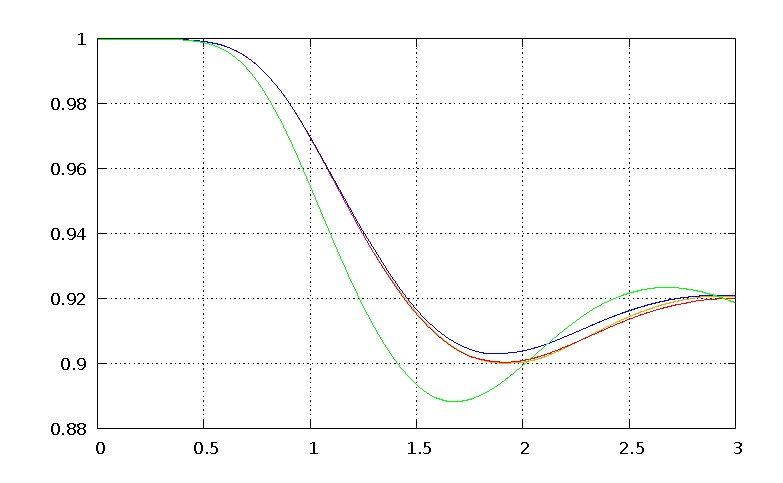
\includegraphics[width=.45\textwidth]
{figures/rising_bubble_I_sphericity.ps}
\caption[Navier--Stokes rising bubble I sphericity]
{A plot of the sphericity $\strikes$ over time for the simulation in
Figure~\ref{fig:risingbubbleIpressure} for the explicit (orange), implicit
(red), ALE (blue) and antisymmetric (green) schemes.}
\label{fig:risingbubbleIsphericity}
\end{figure}

\begin{figure}[htbp]
\centering
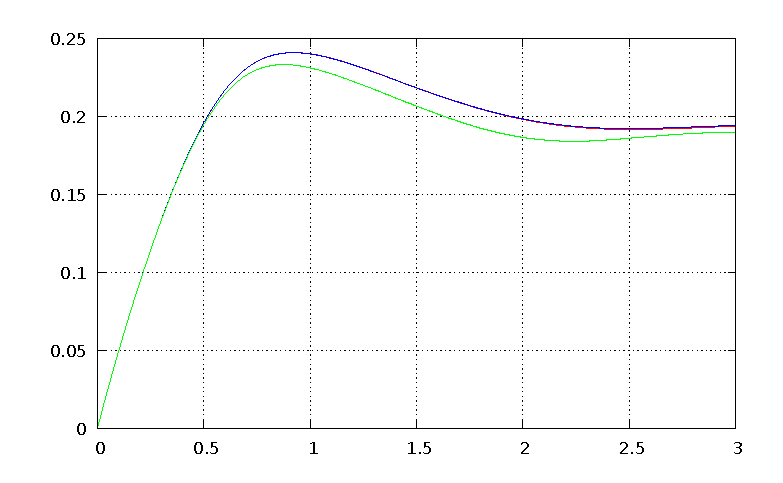
\includegraphics[width=.45\textwidth]
{figures/rising_bubble_I_rising_velocity.ps}
\caption[Navier--Stokes rising bubble I rising velocity]
{A plot of the rising velocity $V_c$ over time for the simulation in
Figure~\ref{fig:risingbubbleIpressure} for the explicit (orange), implicit
(red), ALE (blue) and antisymmetric (green) schemes.}
\label{fig:risingbubbleIrisingvelocity}
\end{figure}

\begin{figure}[htbp]
\centering
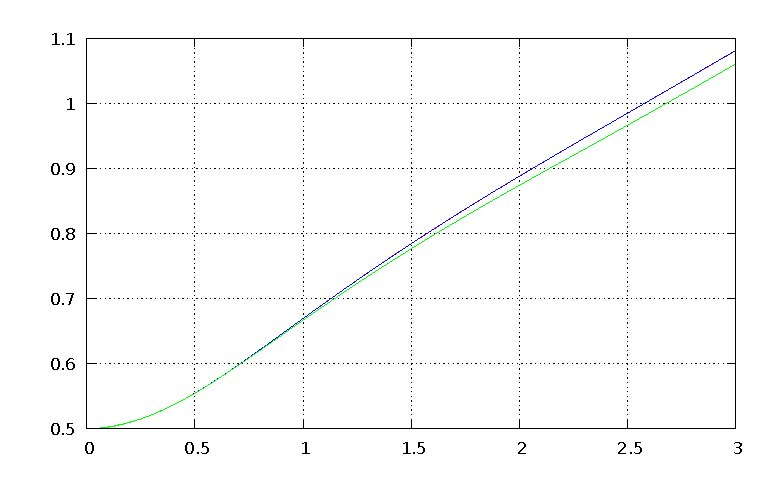
\includegraphics[width=.45\textwidth]
{figures/rising_bubble_I_barycenter.ps}
\caption[Navier--Stokes rising bubble I barycenter]
{A plot of the barycenter $z_c$ over time for the simulation in
Figure~\ref{fig:risingbubbleIpressure} for the explicit (orange), implicit
(red), ALE (blue) and antisymmetric (green) schemes.}
\label{fig:risingbubbleIbarycenter}
\end{figure}

\begin{figure}[htbp]
\centering
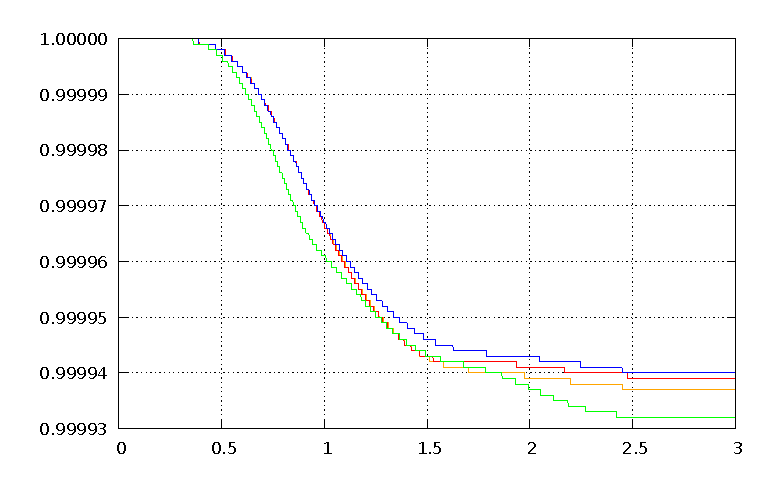
\includegraphics[width=.45\textwidth]
{figures/rising_bubble_I_inner_volume.ps}
\caption[Navier--Stokes rising bubble I inner area]
{A plot of the relative inner area
$\frac{\mathcal{L}^2(\Omega^m_-)}{\mathcal{L}^2(\Omega^0_-)}$ over time for the
simulation in Figure~\ref{fig:risingbubbleIpressure} for the explicit
(orange), implicit (red), ALE (blue) and antisymmetric (green) schemes.}
\label{fig:risingbubbleIinnervolume}
\end{figure}

The physical parameters for the rising bubble experiment II are
\begin{equation} \label{eq:Hysing2}
\rho_+ = 10^3\,,\quad \rho_- = 1\,,\quad \mu_+ = 10\,,\quad \mu_- = 0.1\,,\quad
\gamma = 1.96\,,
\end{equation}
see the test case 2 in \cite[Table~I]{HysingTKPBGT09}. We report on
quantitative results for the rising bubble experiment II in
Table~\ref{tab:risingbubbleII}. See \S\ref{sec:benchmark_quantities} for the
definitions of the various benchmark quantities. For each element, we compare
the explicit, implicit and ALE scheme. We use $J_\Gamma=128$ interface elements
with $J_\Omega^0=35\,092$ initial bulk elements. The final number of bulk
elements, $J_\Omega^M$, for the explicit scheme is 10\,638.
\begin{table*}
\center
\hspace*{-3.25cm}
\begin{tabular}{rrrr}
\hline
& ($\schemeAex)$ & $(\schemeAim)$ & $(\schemeALE)$ \\
\hline
$\strikes_{\min}$                & 0.5435 & 0.5473 & 0.5266 \\
$t_{\strikes = \strikes_{\min}}$ & 3.0000 & 3.0000 & 3.0000 \\
$V_{c,\max 1}$                   & 0.2503 & 0.2502 & 0.2502 \\
$t_{V_c = V_{c,\max 1}}$         & 0.7290 & 0.7290 & 0.7300 \\
$V_{c,\max 2}$                   & 0.2403 & 0.2403 & 0.2400 \\
$t_{V_c = V_{c,\max 2}}$         & 2.1070 & 2.1540 & 2.0670 \\
$z_c(t=3)$                       & 1.1383 & 1.1387 & 1.1385 \\
CPU                              & 132\,498 & 236\,635 & 236\,253 \\
\hline
\end{tabular}
\hspace*{-3.25cm}
\caption[Navier--Stokes rising bubble II benchmark values]
{($\rho_+ = 10^3,\rho_- = 1,\mu_+ = 10,\mu_- =0.1,\gamma = 1.96$)
Rising bubble experiment II on $\Omega = (0,1) \times (0,2)$ over the time
interval $[0,3]$, with nearly uniform meshes and $J_\Gamma=128$ interface
elements.}
\label{tab:risingbubbleII}
\end{table*}
We observe that the results in Table~\ref{tab:risingbubbleII}
are in good agreement with the corresponding numbers from the finest
discretization run of group 3 in \cite{HysingTKPBGT09}, which are given by
0.5144, 3.0000, 0.2502, 0.7317, 0.2393, 2.0600 and 1.1376. Here we note that
there is little agreement on these results between the three groups in
\cite{HysingTKPBGT09}, but we believe the numbers of group 3 to be the most
reliable ones. Similar results are also obtained in 
\cite[Tables~5 and 6]{fluidfbp}.
\footnote{Marco: Why not for the antisymmetric scheme? Should mention that.}

In Figure~\ref{fig:risingbubbleIIpressure} we show the evolution of the discrete
pressures for a simulation with $J_\Gamma=128$ interface elements using the
explicit scheme, while the velocities are visualized in
Figure~\ref{fig:risingbubbleIIvelocity}.
\begin{figure}[htbp]
\centering
\subfloat[$t=10^{-1}$]{\includegraphics[width=.45\textwidth]
{figures/rising_bubble_II_pressure_0.ps}}
\subfloat[$t=1$]{\includegraphics[width=.45\textwidth]
{figures/rising_bubble_II_pressure_1.ps}}\\
\subfloat[$t=2$]{\includegraphics[width=.45\textwidth]
{figures/rising_bubble_II_pressure_2.ps}}
\subfloat[$t=3$]{\includegraphics[width=.45\textwidth]
{figures/rising_bubble_II_pressure_3.ps}}
\caption[Navier--Stokes rising bubble II pressure]
{($\rho_+ = 10^3,\rho_- = 1,\mu_+ = 10,\mu_- =0.1,\gamma = 1.96$)
Pressure evolution for the rising bubble experiment II for the explicit scheme,
with nearly uniform mesh and $J_\Gamma=128$ interface elements.}
\label{fig:risingbubbleIIpressure}
\end{figure}

\begin{figure}[htbp]
\centering
\subfloat[$t=10^{-1}$]{\includegraphics[width=.45\textwidth]
{figures/rising_bubble_II_velocity_0.ps}}
\subfloat[$t=1$]{\includegraphics[width=.45\textwidth]
{figures/rising_bubble_II_velocity_1.ps}}\\
\subfloat[$t=2$]{\includegraphics[width=.45\textwidth]
{figures/rising_bubble_II_velocity_2.ps}}
\subfloat[$t=3$]{\includegraphics[width=.45\textwidth]
{figures/rising_bubble_II_velocity_3.ps}}
\caption[Navier--Stokes rising bubble II velocity]
{Velocity vector field for the simulation in
Figure~\ref{fig:risingbubbleIIpressure}.}
\label{fig:risingbubbleIIvelocity}
\end{figure}

In Figures~\ref{fig:risingbubbleIIsphericity},
\ref{fig:risingbubbleIIrisingvelocity}, \ref{fig:risingbubbleIIbarycenter} and
\ref{fig:risingbubbleIIinnervolume} are reported, respectively, the evolution of
the sphericity $\strikes$, rising velocity $V_c$, barycenter $z_c$ and relative
inner area $\frac{\mathcal{L}^2(\Omega^m_-)}{\mathcal{L}^2(\Omega^0_-)}$ over
time. In Figure~\ref{fig:risingbubbleIIinnervolume} we observe oscillations in
the relative inner area between $t=2.1$ and $t=2.3$. In that interval the bubble
assumes a more non-convex shape and develops thin filaments which originate
these oscillations.
\begin{figure}[htbp]
\centering
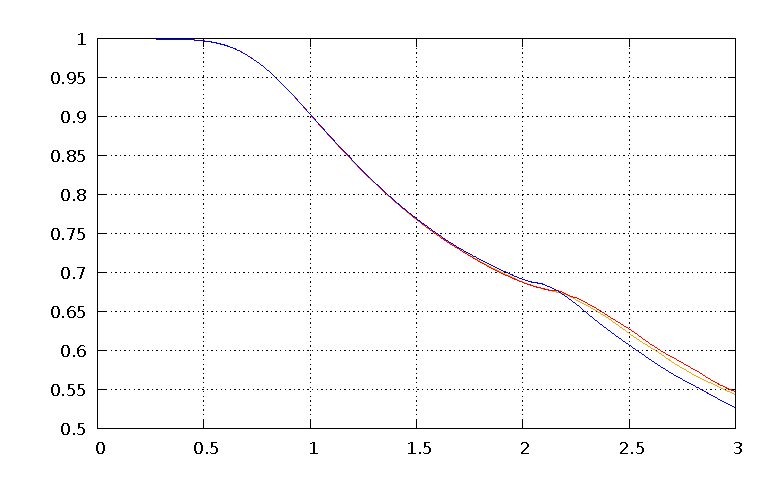
\includegraphics[width=.45\textwidth]
{figures/rising_bubble_II_sphericity.ps}
\caption[Navier--Stokes rising bubble II sphericity]
{A plot of the sphericity $\strikes$ over time for the simulation in
Figure~\ref{fig:risingbubbleIIpressure} for the explicit (orange), implicit
(red) and ALE (blue) schemes.}
\label{fig:risingbubbleIIsphericity}
\end{figure}

\begin{figure}[htbp]
\centering
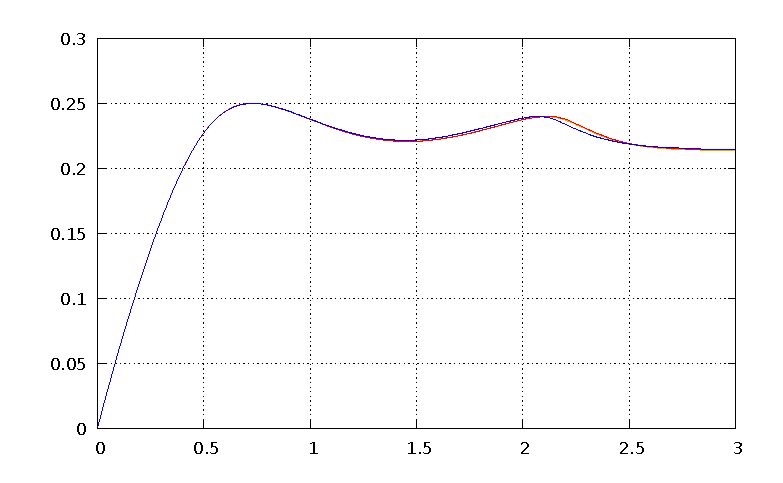
\includegraphics[width=.45\textwidth]
{figures/rising_bubble_II_rising_velocity.ps}
\caption[Navier--Stokes rising bubble II rising velocity]
{A plot of the rising velocity $V_c$ over time for the simulation in
Figure~\ref{fig:risingbubbleIIpressure} for the explicit (orange), implicit
(red) and ALE (blue) schemes.}
\label{fig:risingbubbleIIrisingvelocity}
\end{figure}

\begin{figure}[htbp]
\centering
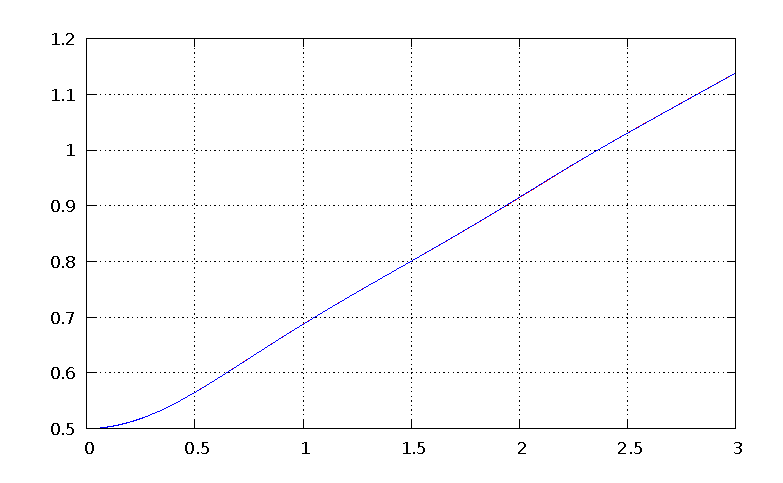
\includegraphics[width=.45\textwidth]
{figures/rising_bubble_II_barycenter.ps}
\caption[Navier--Stokes rising bubble II barycenter]
{A plot of the barycenter $z_c$ over time for the simulation in
Figure~\ref{fig:risingbubbleIIpressure} for the explicit (orange), implicit
(red) and ALE (blue) schemes.}
\label{fig:risingbubbleIIbarycenter}
\end{figure}

\begin{figure}[htbp]
\centering
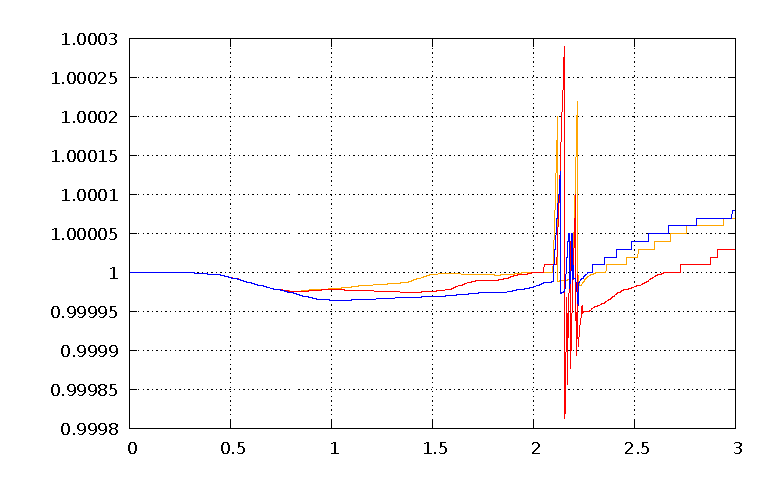
\includegraphics[width=.45\textwidth]
{figures/rising_bubble_II_inner_volume.ps}
\caption[Navier--Stokes rising bubble II inner area]
{A plot of the relative inner area
$\frac{\mathcal{L}^2(\Omega^m_-)}{\mathcal{L}^2(\Omega^0_-)}$ over time for the
simulation in Figure~\ref{fig:risingbubbleIIpressure} for the explicit
(orange), implicit (red) and ALE (blue) schemes.}
\label{fig:risingbubbleIIinnervolume}
\end{figure}

We finally notice that in both experiments, namely the rising bubble I and II,
the ALE scheme and the non-ALE schemes are all performing well. Therefore, the
downside of having to project the velocity in the non-ALE formulations seems to
be less severe than expected. This can be partly explained by the good
interface mesh, which never changes even after a full bulk remeshing.

\section*{Conclusions}
\footnote{TODO}

\bibliographystyle{siam}
\bibliography{../../bib/robert_refs,../../bib/marco_refs}
\end{document}
